\documentclass{article}
\pdfoutput=1

\newif\ifarxiv
\arxivtrue

\ifarxiv
\else
\usepackage{iclr2023_conference,times}
% \documentclass[11pt]{article} % arxiv
\fi

% Recommended, but optional, packages for figures and better typesetting:
\usepackage{microtype}
\usepackage{graphicx}
\usepackage{subfigure}
\usepackage{booktabs} % for professional tables
\usepackage{amssymb}
\usepackage{bm}
\usepackage{bbm}
\usepackage{amsmath}  % Define \boldsymbol (in amsbsy too) and align
\usepackage{amsthm}
\usepackage{xcolor}
\usepackage{textcomp}
\usepackage{multirow}
\usepackage{mathtools}
\usepackage{algorithm}
\usepackage{algorithmic}
\usepackage{xspace}
\ifarxiv
\usepackage[sort,numbers]{natbib}
\usepackage[margin=1in]{geometry} % arxiv
\fi

% Make Figure caption smaller: https://tex.stackexchange.com/questions/86120/font-size-of-figure-caption-header
% https://tex.stackexchange.com/questions/94016/how-to-reduce-space-between-image-and-its-caption
% https://tex.stackexchange.com/questions/94028/how-to-remove-space-between-table-and-caption
\usepackage{caption}
\captionsetup[figure]{skip=1pt,font=small}
\captionsetup[table]{skip=1pt,font=small}

\usepackage{tikz}
\usetikzlibrary{arrows}
\usetikzlibrary{positioning}

\tikzset{
  treenode/.style = {align=center, inner sep=0pt, text centered,
    font=\sffamily},
  arn_n/.style = {treenode, circle, black, font=\sffamily\bfseries, draw=black,
    fill=white, text width=1.5em},% arbre rouge noir, noeud noir
  arn_r/.style = {treenode, circle, black, font=\sffamily\bfseries, draw=black,
    fill=white, text width=1.0em},% arbre rouge noir, noeud rouge
  arn_x/.style = {treenode, rectangle, draw=black,
    minimum width=0.5em, minimum height=0.5em}% arbre rouge noir, nil
}

\definecolor{tabblue}{HTML}{4e79a7}
\definecolor{tabred}{HTML}{e15759}
\usepackage[hidelinks,colorlinks=true,linkcolor=tabred,citecolor=tabblue]{hyperref}
\usepackage{url}

% Attempt to make hyperref and algorithmic work together better:
\newcommand{\theHalgorithm}{\arabic{algorithm}}


% bolded matirx
\usepackage{bm}
\usepackage{enumitem}

\usepackage[capitalise]{cleveref}  % cleveref needs to be loaded after hyperref


\ifarxiv
\else
% --------------------
% Space-saving options
\usepackage[compact]{titlesec}
\titlespacing{\section}{0pt}{*0.3}{*0}
\titlespacing{\subsection}{0pt}{*0.15}{*0}

\usepackage[subtle, mathdisplays=tight, charwidths=tight, leading=normal]{savetrees}
% \usepackage[subtle, mathdisplays=tight, charwidths=normal, leading=normal]{savetrees}
% \usepackage[subtle]{savetrees}

% Can always cheat a bit on the margins
% \addtolength\titlebox{-0.3in}
% \addtolength\columnsep{-0.15in}
\addtolength\textwidth{0.15in}
\addtolength\textheight{0.15in}
\addtolength\textfloatsep{-0.7em}
\addtolength\intextsep{-0.3em}
\fi

% https://tex.stackexchange.com/questions/146890/how-to-apply-looseness-1-to-all-the-paragraphs
% Does savetrees do this already?
% \linepenalty=1000

\def\setstretch#1{\renewcommand{\baselinestretch}{#1}}
\setstretch{0.985}
\addtolength{\parskip}{-1pt}

\newcommand{\diag}{\mathrm{diag}}
\newcommand{\softmax}{\mathrm{softmax}}
\newcommand{\Sim}{\mathrm{Sim}}
\newcommand{\defeq}{:=}

\newcommand{\vA}{\mathbf{A}}
\newcommand{\vB}{\mathbf{B}}
\newcommand{\vC}{\mathbf{C}}
\newcommand{\vD}{\mathbf{D}}
\newcommand{\vE}{\mathbf{E}}
\newcommand{\vF}{\mathbf{F}}
\newcommand{\vI}{\mathbf{I}}
\newcommand{\vQ}{\mathbf{Q}}
\newcommand{\vK}{\mathbf{K}}
\newcommand{\vV}{\mathbf{V}}
\newcommand{\vdQ}{\mathbf{dQ}}
\newcommand{\vdK}{\mathbf{dK}}
\newcommand{\vdV}{\mathbf{dV}}
\newcommand{\vS}{\mathbf{S}}
\newcommand{\vdS}{\mathbf{dS}}
\newcommand{\vP}{\mathbf{P}}
\newcommand{\vdP}{\mathbf{dP}}
\newcommand{\vU}{\mathbf{U}}
\newcommand{\vW}{\mathbf{W}}
\newcommand{\vT}{\mathbf{T}}
\newcommand{\vX}{\mathbf{X}}
\newcommand{\vO}{\mathbf{O}}
\newcommand{\vdO}{\mathbf{dO}}
\newcommand{\vM}{\mathbf{M}}
\newcommand{\vZ}{\mathbf{Z}}

% \newcommand*{\ShowNotes}{}
\newcommand{\ctask}{c_{\text{task}}}
\newcommand{\cmodel}{c_{\text{model}}}

\newcommand{\ms}{\mathscr}
\newcommand{\mc}{\mathcal}
\newcommand{\mf}{\mathfrak}

\newcommand{\bs}{\backslash}
\newcommand{\nsg}{\unlhd}
\newcommand{\ov}{\overline}

\newcommand{\N}{\mathbb{N}}
\newcommand{\R}{\mathbb{R}}
\newcommand{\Z}{\mathbb{Z}}
\newcommand{\Q}{\mathbb{Q}}
\newcommand{\F}{\mathbb{F}}
\newcommand{\C}{\mathbb{C}}

\newcommand{\Zp}{\Z^+}

\newcommand{\Rom}{\R^\omega}
\newcommand{\Rinf}{\R^\infty}

\newcommand{\linf}{\ell_\infty}
\newcommand{\lp}{\ell_p}
\newcommand{\lone}{\ell_1}

\newcommand{\dinf}{d_\infty}

\newcommand{\hess}{\nabla^2}
\newcommand{\diag}{\text{diag}}

\newcommand{\blone}{\textbf{1}}

\newcommand{\omn}{\omega_n}


\newcommand{\ip}{\langle\,,\rangle}

\newcommand{\mcP}{\mc{P}}
\newcommand{\mcS}{\mc{S}}
\newcommand{\mcB}{\mc{B}}
\newcommand{\mcC}{\mc{C}}
\newcommand{\mcF}{\mc{F}}
\newcommand{\mcI}{\mc{I}}
\newcommand{\mcE}{\mc{E}}
\newcommand{\mcA}{\mc{A}}
\newcommand{\mcL}{\mc{L}}


\newcommand{\aln}{{\aleph_0}}

\newcommand{\Rn}{\mathbb{R}^n}
\newcommand{\Rnn}{\R^{n \times n}}
\newcommand{\eps}{\epsilon}
\newcommand{\norm}[1]{||#1||}
\newcommand{\pnorm}[1]{\norm{#1}_p}
\newcommand{\qnorm}[1]{\norm{#1}_q}
\newcommand{\onorm}[1]{\norm{#1}_1}
\newcommand{\inorm}[1]{||#1||_\infty}
\newcommand{\tnorm}[1]{\norm{#1}_2}
\newcommand{\shyone}[1]{\frac{#1}{#1}}
\newcommand{\shyzero}[1]{#1 - #1}
\newcommand{\floor}[1]{\left\lfloor #1 \right\rfloor}
\newcommand{\ceil}[1]{\left\lceil #1 \right\rceil}
\newcommand{\pd}[1]{\frac{\partial}{\partial #1}}
\newcommand{\pdn}[2]{\frac{\partial^{#2}}{\partial {#1}^{#2}}}
\newcommand{\pdm}[2]{\frac{\partial^{#2}}{\partial {#1}}}
\newcommand{\diex}{\pd{x}}
\newcommand{\diey}{\pd{y}}
\newcommand{\diez}{\pd{z}}
\newcommand{\ddx}{\frac{d}{dx}}
\newcommand{\mat}[1]{\begin{bmatrix} #1 \end{bmatrix}}
\newcommand{\EX}{\mathbb{E}}
\newcommand{\Var}[1]{\text{Var}(#1)}
\newcommand{\recip}[1]{\frac{1}{#1}}
\newcommand{\inv}[1]{#1^{-1}}
\newcommand{\finv}{\inv{f}}
\newcommand{\set}[1]{\{#1\}}
\newcommand{\braces}[1]{\left\{ #1 \right\}}
\newcommand{\setstar}[1]{\{#1\}^*}
\newcommand{\jjlim}[2]{\lim_{#2 \rightarrow #1}}
\newcommand{\jjpar}[1]{\left( #1 \right)}
\newcommand{\jjbra}[1]{\left\{ #1 \right\}}
\newcommand{\jjabs}[1]{\left\lvert #1 \right\rvert}
\newcommand{\jjcases}[1]{\begin{cases} #1 \end{cases}}
\newcommand{\jjalg}[2]{ 
    
    \noindent {#1}
        \begin{algorithmic}[1]
            #2
        \end{algorithmic}
}
\newcommand{\jjbold}[1]{{\bf #1}}


\newcommand{\LT}[1]{\mathcal{L}\set{#1}}
\newcommand{\LTi}[1]{\mathcal{L}^{-1}\set{#1}}

\newcommand{\ket}[1]{\left\lvert #1 \right\rangle}
\newcommand{\kphi}{\ket{\phi}}
\newcommand{\kpsi}{\ket{\psi}}
\newcommand{\kOmega}{\ket{\Omega}}
\newcommand{\kone}{\ket{1}}
\newcommand{\koone}{\ket{11}}
\newcommand{\kzero}{\ket{0}}
\newcommand{\kzzero}{\ket{00}}
\newcommand{\kzone}{\ket{01}}
\newcommand{\kozero}{\ket{10}}

\newcommand{\bra}[1]{\left\langle #1 \right\rvert}
\newcommand{\bphi}{\bra{\phi}}
\newcommand{\bpsi}{\bra{\psi}}
\newcommand{\bOmega}{\bra{\Omega}}
\newcommand{\bone}{\bra{1}}
\newcommand{\boone}{\bra{11}}
\newcommand{\bzero}{\bra{0}}
\newcommand{\bzzero}{\bra{00}}
\newcommand{\bzone}{\bra{01}}
\newcommand{\bozero}{\bra{10}}


\newcommand{\matX}{\mat{0 & 1 \\ 1 & 0}}
\newcommand{\matY}{\mat{0 & -i \\ i & 0}}
\newcommand{\matZ}{\mat{1 & 0 \\ 0 & -1}}
\newcommand{\matH}{\irtwo\mat{1 & 1 \\ 1 & -1}}
\newcommand{\matI}{\mat{1 & 0 \\ 0 & 1}}
\newcommand{\matCNOT}{\mat{1 & 0 & 0 & 0 \\ 0 & 1 & 0 & 0 \\ 0 & 0 & 0 & 1 \\ 0 & 0 & 1 & 0}}
\newcommand{\matUCNOT}{\mat{1 & 0 & 0 & 0 \\ 0 & 0 & 0 & 1 \\ 0 & 0 & 1 & 0 \\ 0 & 1 & 0 & 0}}


\newcommand{\rt}{\sqrt{2}}
\newcommand{\half}{\frac{1}{2}}
\newcommand{\third}{\frac{1}{3}}
\newcommand{\tthird}{\frac{2}{3}}
\newcommand{\fourth}{\frac{1}{4}}
\newcommand{\fifth}{\frac{1}{5}}
\newcommand{\sixth}{\frac{1}{6}}
\newcommand{\seventh}{\frac{1}{7}}
\newcommand{\eighth}{\frac{1}{8}}


\newcommand{\irtwo}{\frac{1}{\sqrt{2}}}
\newcommand{\irtwoa}[1]{\frac{#1}{\sqrt{2}}}
\newcommand{\itrtwo}{\frac{1}{2\sqrt{2}}}


\newcommand{\jjdag}[1]{#1^\dagger}

\newcommand{\softmax}[1]{\text{softmax}\jjpar{#1}}
\newcommand{\SDP}[1]{\text{SDP}\jjpar{#1}}
\newcommand{\LSE}[1]{\text{LSE}\jjpar{#1}}

\newcommand{\seqlen}{\text{seqlen}}

\title{Hungry Hungry Hippos: Towards Language Modeling with State Space Models}

\ifarxiv
  \usepackage{authblk}
  \author[$\dagger$]{Daniel Y. Fu\thanks{Equal Contribution. Order determined by coin flip.}}
  \author[$\dagger$]{Tri Dao$^*$}
  \author[$\ddagger$]{Khaled K. Saab}
  \author[$\dagger\dagger$]{Armin W. Thomas}
  \author[$\ddagger\ddagger$]{\\ Atri Rudra}
  \author[$\dagger$]{Christopher R{\'e}}
  \affil[$\dagger$]{Department of Computer Science, Stanford University}
  \affil[$\ddagger$]{Department of Electrical Engineering, Stanford University}
  \affil[$\dagger\dagger$]{Department of Psychology, Stanford University}
  \affil[$\ddagger\ddagger$]{Department of Computer Science and Engineering, University at Buffalo, SUNY\vspace{4pt}}
  \affil[ ]{{\texttt{\{danfu,tridao\}@cs.stanford.edu}, \texttt{\{ksaab,athms\}@stanford.edu}, \texttt{atri@buffalo.edu}, \texttt{chrismre@cs.stanford.edu}}}

  \date{December 28, 2022}

\else

\author{Daniel Y. Fu\thanks{Equal Contribution. Order determined by coin flip.}~$^{~\dagger}$, Tri Dao$^{* \dagger}$, Khaled K. Saab$^{\dagger}$, Armin W. Thomas$^{\dagger}$, Atri Rudra$^{\ddagger}$, Christopher R\'{e}$^{\dagger}$ \\
$\dagger$ Stanford University, $\ddagger$ University at Buffalo, SUNY \\
\texttt{\{danfu,tridao\}@cs.stanford.edu},~\texttt{\{ksaab,athms\}@stanford.edu}, \\
\texttt{atri@buffalo.edu},~\texttt{chrismre@cs.stanford.edu}
}
% iclr authors

\fi

% iclr stuff
\newcommand{\fix}{\marginpar{FIX}}
\newcommand{\new}{\marginpar{NEW}}
% iclr stuff
\ifarxiv
\else
\iclrfinalcopy % Uncomment for camera-ready version, but NOT for submission.
\fi
\begin{document}

\maketitle

% for compiling before there's content
% \nocite{*}

\begin{abstract}
  \begin{abstract}
There is a widely-spread claim that GANs are difficult to train, and GAN architectures in the literature are littered with empirical tricks. We provide evidence against this claim and build a modern GAN baseline in a more principled manner. First, we derive a well-behaved regularized relativistic GAN loss that addresses issues of mode dropping and non-convergence that were previously tackled via a bag of ad-hoc tricks. We analyze our loss mathematically and prove that it admits local convergence guarantees, unlike most existing relativistic losses. Second, this loss allows us to discard all ad-hoc tricks and replace outdated backbones used in common GANs with modern architectures. Using StyleGAN2 as an example, we present a roadmap of simplification and modernization that results in a new minimalist baseline---\modelName (``Re-GAN''). Despite being simple, our approach surpasses StyleGAN2 on FFHQ, ImageNet, CIFAR, and Stacked MNIST datasets, and compares favorably against state-of-the-art GANs and diffusion models.\\
Code: \href{https://www.github.com/brownvc/R3GAN}{https://www.github.com/brownvc/R3GAN}
\end{abstract}
\end{abstract}

\section{Introduction}
\label{sec:intro}


Transformers, in particular decoder-only models (e.g.\ GPT~\citep{brown2020language}, Llama~\citep{touvron2023llama}) which process input sequences in a causal fashion, are one of the main drivers of modern deep learning's success.
Numerous approaches attempt to approximate the core attention layer to address its efficiency issues~\citep{tay2022efficient}, such as scaling quadratically in sequence length during training and requiring a cache of size linear in sequence length during autoregressive generation.
In parallel, a class of alternative sequence models, structured state-space models (SSMs), have emerged with linear scaling in sequence length during training and constant state size during generation.
They show strong performance on long-range tasks (e.g. S4~\citep{gu2022efficiently}) and recently matched or beat Transformers on language modeling (e.g. Mamba \citep{gu2023mamba}) at small to moderate scale.
However, the development of SSMs have appeared disjoint from the community's collective effort to improve Transformers, such as understanding them theoretically as well as optimizing them on modern hardware.
As a result, it is more difficult to understand and experiment with SSMs compared to Transformers, and it remains challenging to train SSMs as efficiently as Transformers from both an algorithmic and systems perspective.


Our main goal is to develop a rich body of theoretical connections between structured SSMs and variants of attention.
This will allow us to transfer algorithmic and systems optimizations originally developed for Transformers to SSMs, towards the goal of building foundation models that perform better than Transformers while scaling more efficiently in sequence length.
A milestone contribution in this direction was the \textbf{Linear Attention (LA)} framework \citep{katharopoulos2020transformers},
which derived a connection between autoregressive attention and linear RNNs
by showing the equivalence between ``dual forms'' of quadratic kernelized attention and a particular linear recurrence.
This duality allows new capabilities such as the ability to have both efficient parallelizable training and efficient autoregressive inference.
In the same spirit, this paper provides multiple viewpoints connecting linear-complexity SSMs with quadratic-complexity forms to combine the strengths of SSMs and attention.%
\footnote{Technically speaking, these connections only relate to certain flavors of attention; the title of this paper is an homage to \citet{katharopoulos2020transformers} which first showed that ``Transformers are RNNs''.}

\iftoggle{arxiv}{
\begin{wrapfigure}{R}{0.48\linewidth}
  \begin{center}
    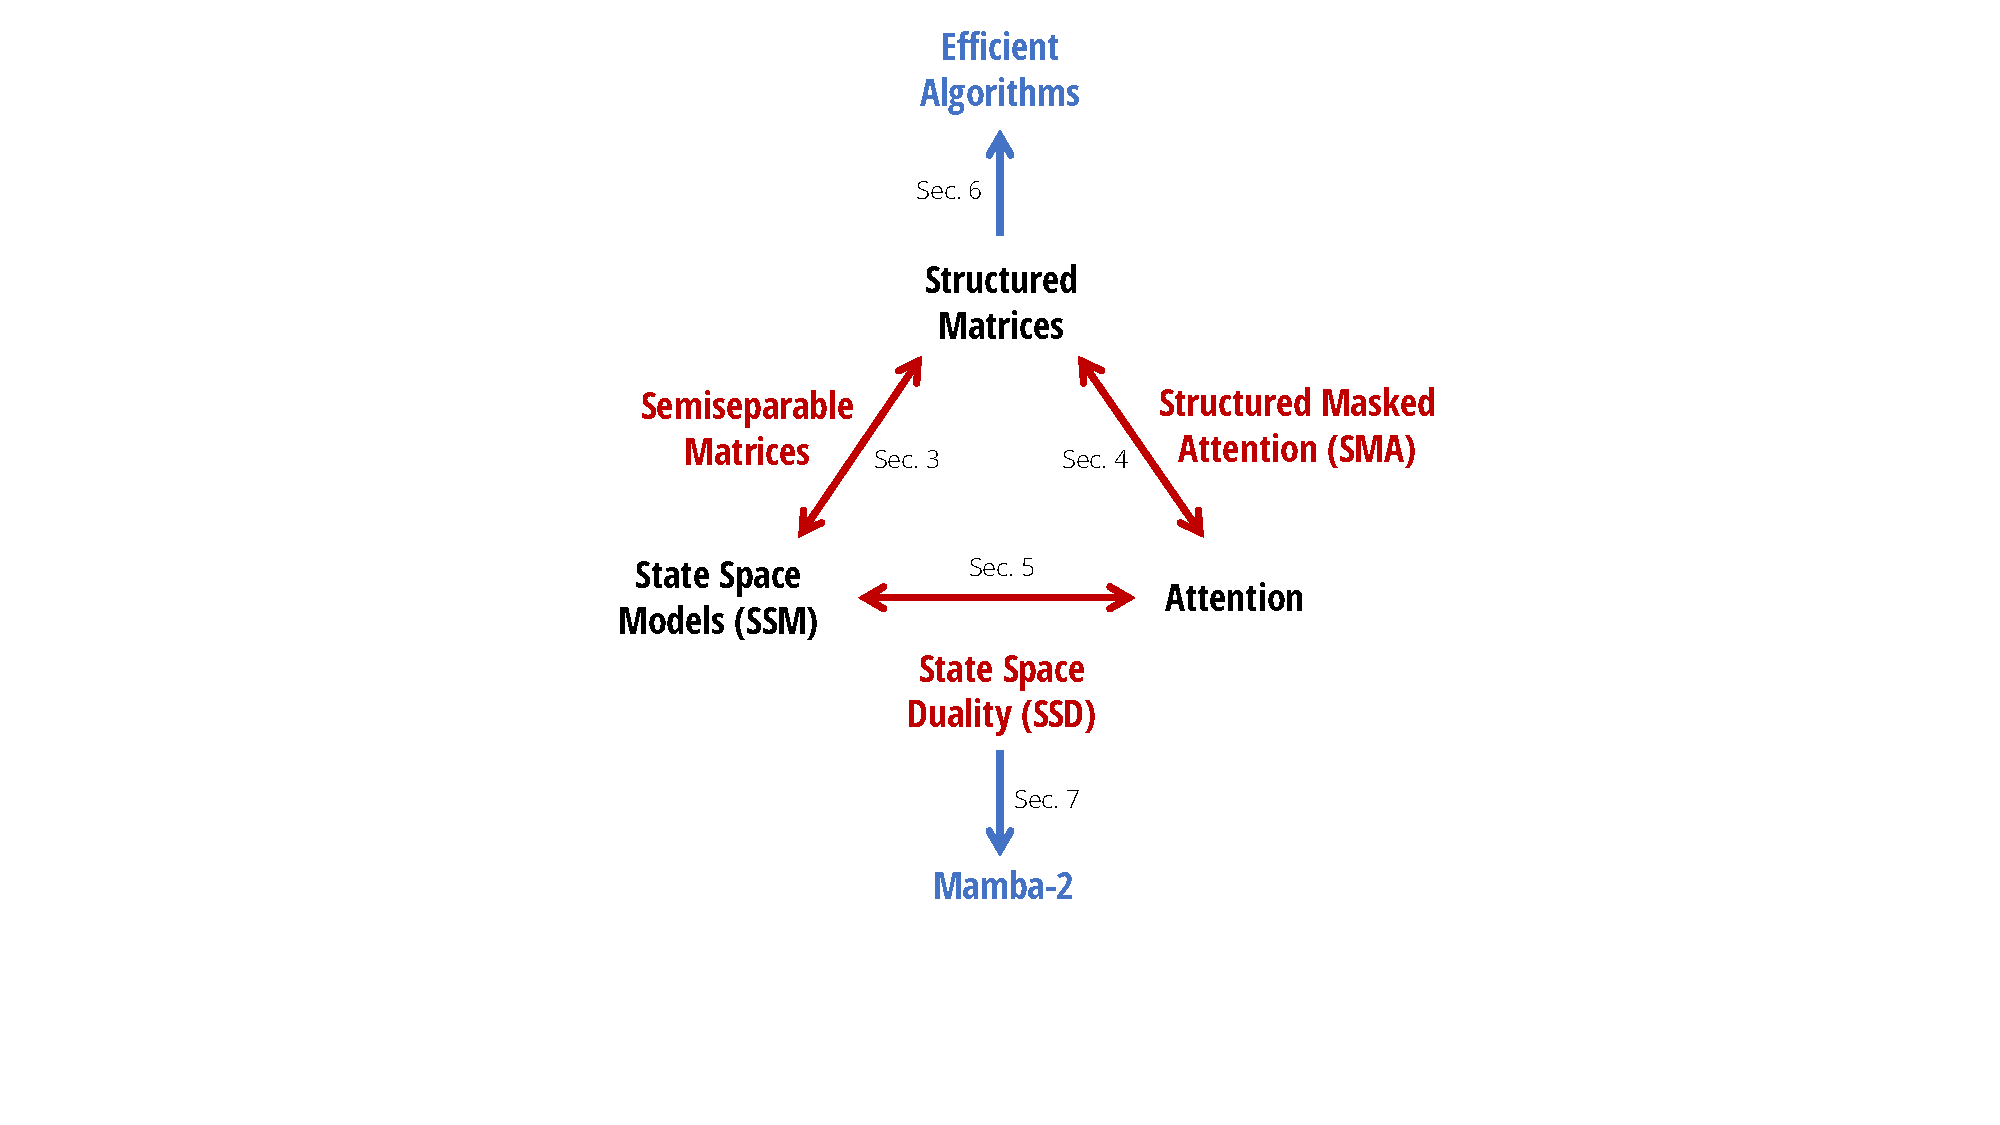
\includegraphics[width=\linewidth]{fig/ssd_roadmap.pdf}
  \end{center}
  \caption{
    (\textbf{Structured State-Space Duality}.)
    This paper fleshes out the relationship between state space models and attention through the bridge of structured matrices.
  }
  \label{fig:roadmap}
\end{wrapfigure}
}{}

\para{State Space Duality.}
Our framework connecting structured SSMs and variants of attention, which we call \textbf{structured state space duality} (SSD),
is made through the abstractions of \textbf{structured matrices}:
matrices with subquadratic parameters and multiplication complexity.
We develop two broad frameworks for representing sequence models, one as matrix transformations and one as tensor contractions, which each reveal different perspectives of the duality.
Our technical contributions include:
\begin{itemize}[leftmargin=*,itemsep=0pt,topsep=0pt]
  \item We show an equivalence between state space models and a well-studied family of structured matrices called \textbf{semiseparable matrices}\iftoggle{arxiv}{ (\cref{sec:ssm})}{}.
    This connection is at the heart our framework, revealing new properties and algorithms for SSMs. A central message of this paper is that \emph{different methods of computing state space models can be reframed as various matrix multiplication algorithms on structured matrices}.
  \item We significantly improve the theory of linear attention~\citep{katharopoulos2020transformers}.
    We first provide an incisive proof of its recurrent form through the language of tensor contractions, and then generalize it to a new family of \textbf{structured masked attention (SMA)}\iftoggle{arxiv}{ (\cref{sec:attention})}{}.
  \item We connect SSMs and SMA, showing that they have a large intersection that are duals of each other, possessing both SSM-like linear and attention-like quadratic forms\iftoggle{arxiv}{ (\cref{sec:ssd})}{}.
    \iftoggle{arxiv}{We also prove that any kernel attention method possessing a fast recurrent form must be an SSM.}{}
\end{itemize}


Beyond its intrinsic theoretical value, our framework opens up a broad set of directions for understanding and improving sequence models.

\para{Efficient Algorithms.}
First and most importantly, our framework exposes new efficient and easily-implementable algorithms for computing SSMs\iftoggle{arxiv}{ (\cref{sec:efficient})}{}.
We introduce a new \textbf{SSD algorithm}, based on block decompositions of semiseparable matrices, that takes advantage of both the linear SSM recurrence and quadratic dual form, obtaining optimal tradeoffs on all main efficiency axes (e.g. training and inference compute, memory usage, and ability to leverage matrix multiplication units on modern hardware).
A dedicated implementation of SSD is $2-8\times$ faster than the optimized selective scan implementation of Mamba, while simultaneously allowing for much larger recurrent state sizes ($8\times$ the size of Mamba or even higher, with minimal slowdown).
SSD is highly competitive with optimized implementations of softmax attention (FlashAttention-2~\citep{dao2023flashattention2}), crossing over at sequence length 2K and 6$\times$ faster at sequence length 16K.


\iftoggle{arxiv}{
\para{Architecture Design.}
One major obstacle to adopting new architectures such as SSMs is the ecosystem tailored to Transformers, such as hardware-efficient optimization and parallelism techniques for large-scale training.
Our framework allows using established conventions and techniques for attention to build a vocabulary of architecture design choices for SSMs, and further improve them (\cref{sec:architecture}).
For example, we introduce the analog of heads from multi-head attention (MHA) to SSMs.
We show that the Mamba architecture is a \textbf{multi-input SSM (MIS)} that turns out to be analogous to \textbf{multi-value attention (MVA)}, and compare other variants of Mamba with different head structures.

We also use these ideas to make slight modifications to the Mamba block, which allows tensor parallelism to be implemented (e.g. in the style of Megatron~\citep{shoeybi2019megatron}).
The main ideas include introducing grouped-value attention (GVA) head structure, and moving all data-dependent projections to occur in parallel at the beginning of the block.


}{
  \para{Mamba-2.}
  Additionally, inspired by the connection between SSMs and Transformers, we slightly modify the neural network architecture of Mamba by moving all data-dependent projections to occur in parallel at the beginning of the block. %
}
The combination of the modified parallel Mamba block, together with using SSD as the inner SSM layer, results in the \textbf{Mamba-2} architecture.
We investigate Chinchilla scaling laws for Mamba-2 in the same setting as Mamba, finding that it Pareto dominates Mamba and Transformer++ in both perplexity and wall-clock time.
We additionally train a family of Mamba-2 models at varying sizes on the Pile, showing that it matches or outperforms Mamba and open source Transformers on standard downstream evaluations.
For example, Mamba-2 with 2.7B parameters trained on 300B tokens on the Pile outperforms Mamba-2.8B, Pythia-2.8B and even Pythia-6.9B trained on the same dataset.

\iftoggle{arxiv}{
\paragraph{Systems Optimizations.}
The SSD framework connects SSMs and Transformers, allowing us to leverage a rich body of work on systems optimizations developed for Transformers~(\cref{sec:systems}).
\begin{itemize}[leftmargin=*,itemsep=0pt,topsep=0pt]
  \item For example, Tensor Parallelism (TP) is an important model parallelism technique to train large Transformer models by splitting each layer across GPUs on the same node.
    We design Mamba-2 to be TP-friendly, reducing the number of synchronization point per block by half.
  \item For very long sequences whose activations do not fit on one device, sequence parallelism has been developed for the attention blocks.
    We describe how to train SSMs in general and Mamba-2 in particular with sequence parallelism, by passing the recurrent states between devices.
  \item For finetuning with examples of different lengths, for best efficiency, Transformer requires sophisticated techniques to remove padding tokens and perform attention on variable length sequences.
    We show how Mamba-2 can be trained with variable sequence lengths efficiently, requiring no padding tokens.
\end{itemize}
}{}

\cref{sec:experiments} empirically validates Mamba-2 on language modeling, training efficiency, and a difficult multi-query associative recall task~\citep{arora2024simple}.
Finally, in \cref{sec:related}, we provide an extended related work and discuss potential research directions opened up by our framework.

Model code and pre-trained checkpoints are open-sourced at \url{https://github.com/state-spaces/mamba}.






\subsection{Data Augmentation in NLP}
The problem of domain adaptation and OOD robustness is well established in NLP \citep{blitzer-etal-2007-biographies,daume-iii-2007-frustratingly,hendrycks2020pretrained}.
Existing work on improving generalization has focused on data augmentation, where synthetically generated training examples are used to augment an existing dataset.
It is hypothesized that these examples induce robustness to local perturbations, which has been shown to be effective in semi-supervised and self-supervised settings \citep{bachman2014learning,szegedy2014intriguing, sajjadi2016regularization}.

Existing task-specific methods \citep{kafle-etal-2017-data} and word-level methods \citep{zhang2015character, xie2017data, wei-zou-2019-eda} are based on human-designed heuristics.
Back-translation from or through another language has been applied in the context of machine translation \citep{sennrich2016improving}, question answering \citep{wei2018fast}, and consistency training \citep{xie2019unsupervised}.
More recent work has used word embeddings \citep{wangyang2015thats} and LSTM language models \citep{fadaee2017data} to perform word replacement.
Other methods focus on fine-tuning contextual language models \citep{kobayashi-2018-contextual,wu2019conditional,kumar20202data} or large generative models \citep{lambada,yang2020g-daug,kumar20202data} to generate synthetic examples.

\subsection{VRM and the Manifold Assumption}
Vicinal Risk Minimization (VRM) \citep{vicinal200olivier} formalizes data augmentation as enlarging the training set support by drawing samples from a \textit{vicinity} of existing training examples.
Typically the vicinity of a training example is defined using dataset-dependent heuristics.
For example, in computer vision, examples are generated using scale augmentation \citep{simonyan2014very}, color augmentation \citep{krizhevsky2012imagenet}, and translation and rotation \citep{Simard1998}.

The \textit{manifold assumption} states that high dimensional data concentrates around a low-dimensional manifold \citep{chapelle2006semi}.
This assumption allows us to define the vicinity of a training example as its \textit{manifold neighborhood}, the portion of the neighborhood that lies on the data manifold.
Recent methods have used the manifold assumption to improve robustness by moving examples towards a decision boundary \citep{kanbak2018geometric}, generating adversarial examples \cite{szegedy2014intriguing,miyato2017virtual}, interpolating between pairs of examples \citep{zhang2018mixup}, or finding affine transforms \citep{paschali2019data}.

\begin{figure}[t!]
\centering
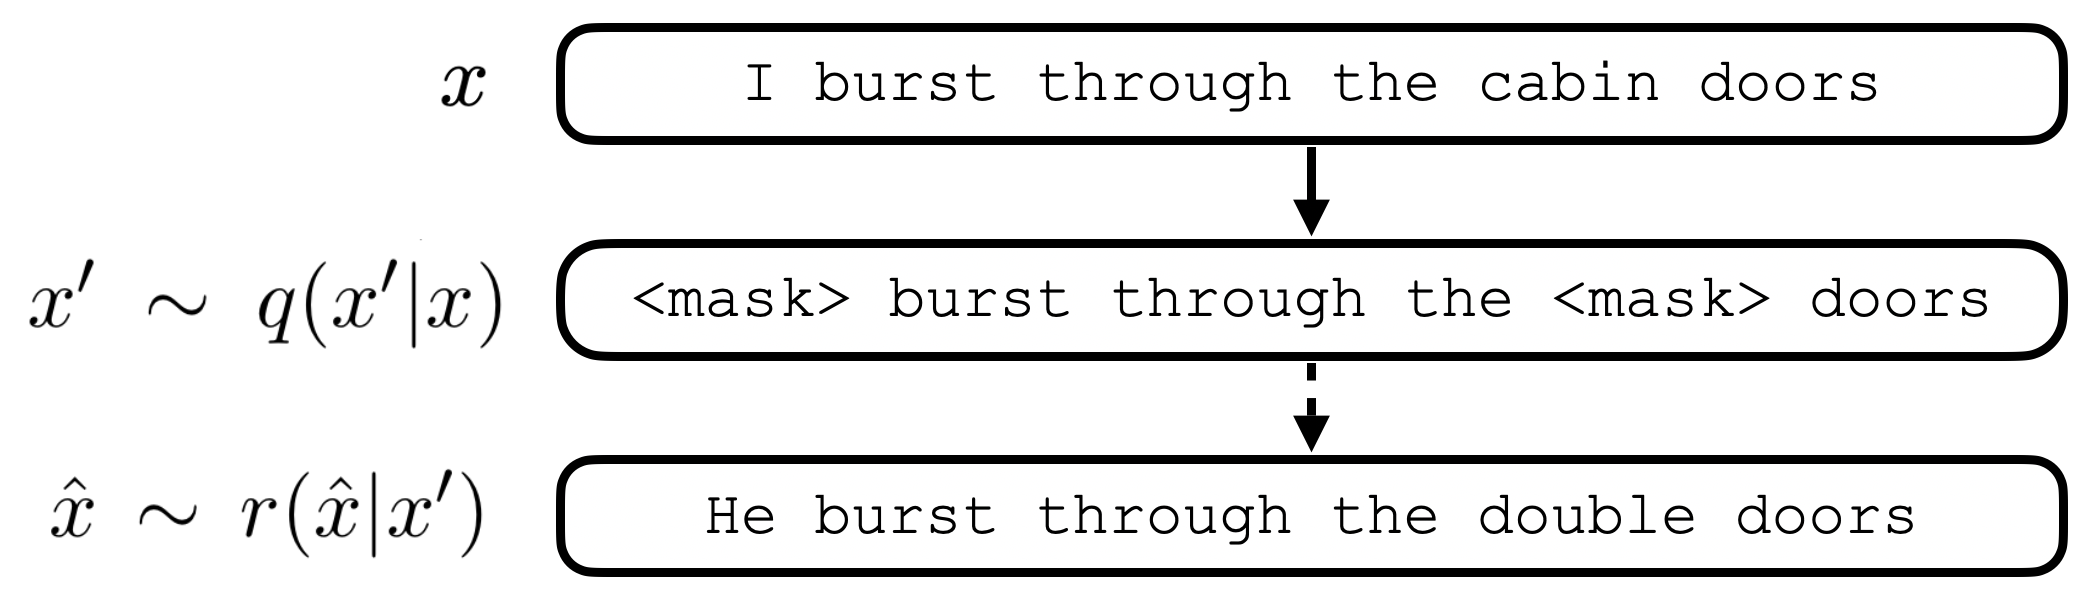
\includegraphics[scale=0.21]{img/bert_dae.png}
\caption{To sample from an MLM DAE, we apply the MLM corruption $q$ to the original sentence then reconstruct the corrupted sentence using our DAE $r$.}
\label{fig:dae_sampling}
\end{figure}

\subsection{Sampling from Denoising Autoencoders}
A denoising autoencoder (DAE) is an autoencoder trained to reconstruct a clean input $x$ from a stochastically corrupted one $x'\sim q(x'|x)$ by learning a conditional distribution $P_\theta (x| x')$ \citep{vincent2008extracting}.
We can sample from a DAE by successively corrupting and reconstructing an input using the following pseudo-Gibbs Markov chain: $x_t' \sim q(x'|x_{t-1})$, $x_t \sim P_\theta(x|x'_t).$
\comment{
\begin{align*}
    x_t' &\sim q(x'|x_{t-1})\\
    x_t &\sim P_\theta(x|x'_t) 
\end{align*}
}
As the number of training examples increases, the asymptotic distribution $\pi_n(x)$ of the generated samples approximate the true data-generating distribution $P(x)$ \citep{bengio2013generalized}.
This corruption-reconstruction process allows for sampling directly along the manifold that $P(x)$ concentrates on.

\subsection{Masked Language Models}
Recent advances in unsupervised representation learning for natural language have relied on pre-training models on a \textit{masked language modeling} (MLM) objective \citep{devlin2018, liu2019roberta}.
In the MLM objective, a percentage of the input tokens are randomly corrupted and the model is asked to reconstruct the original token given its left and right context in the corrupted sentence.
We use MLMs as DAEs \citep{lewis2019bart} to sample from the underlying natural language distribution by corrupting and reconstructing inputs (Figure \ref{fig:dae_sampling}).

% \begin{table}[h]
    % \captionsetup{font=small}
    \small
    \centering
    % \vspace{-1em}
    \caption{\label{table:synthetics} Evaluation of 2-layer models on synthetic language tasks.}
    %   \vspace{1em}
    {
        \begin{tabular}{@{}|c|c|ccc|c|@{}}
        %   \specialrule{.15em}{.05em}{.05em}
        \hline
        Task & Random & S4D & Gated State Spaces & H3 & Attention  \\ % & Training time \\
        %   \specialrule{.15em}{.05em}{.05em}
        \hline
        Induction Head & 5.0 & 35.6 & 6.8 & \textbf{100.0} & \textbf{100.0} \\
        Associative Recall & 25.0 & 86.0 & 78.0 & 99.8 & \textbf{100.0}  \\ \hline
        % Gated State Spaces & 78.0 & 6.8 & 88.2 \\
        % LSTM & -- & -- & -- \\
        % H3 & 99.8 & \textbf{100.0} & \textbf{99.6}  \\ \hline
        % Attention & \textbf{100.0} & \textbf{100.0} & 71.0 \\ \hline
        \end{tabular}
    }
    % \vspace{-1.5em}
\end{table}

% \begin{table}[h]
%     % \captionsetup{font=small}
%     \small
%     \centering
%     % \vspace{-1em}
%     \caption{\label{table:synthetics} Evaluation of 2-layer GPT models on in-context learning synthetic tasks.}
%     %   \vspace{1em}
%     {
%         \begin{tabular}{@{}|c|ccc|@{}}
%         %   \specialrule{.15em}{.05em}{.05em}
%         \hline
%         Model & Associative Recall & Induction Head & Partial Copy  \\ % & Training time \\
%         %   \specialrule{.15em}{.05em}{.05em}
%         \hline
%         Random & 50.0 & 5.0 & 5.0 \\
%         S4D & 86.0 & 35.6 & 98.5  \\
%         Gated State Spaces & 78.0 & 6.8 & 88.2 \\
%         % LSTM & -- & -- & -- \\
%         H3 & 99.8 & \textbf{100.0} & \textbf{99.6}  \\ \hline
%         Attention & \textbf{100.0} & \textbf{100.0} & 71.0 \\ \hline
%         \end{tabular}
%     }
%     % \vspace{-1.5em}
% \end{table}
\section{Methodology}
\ours follows the same framework as speculative decoding, where each decoding step primarily consists of three substeps: (1) generating candidates, (2) processing candidates, and (3) accepting candidates. For \ours, (1) is achieved by \ours heads, (2) is realized by tree attention, and since \ours heads are on top of the original model, the logits calculated in (2) can be used for substep (1) for the next decoding step. The final step (3) can be realized by either rejection sampling~\citep{leviathan2022fast,chen2023accelerating} or typical acceptance (Section~\ref{sec:typical_acceptance}). The overall pipeline is illustrated in Figure~\ref{fig:pipeline}.

In this section, we first introduce the key components of \ours, including \ours heads, and tree attention. Then, we present two levels of fine-tuning procedures for \ours to meet the needs of different use cases. Finally, we propose two extensions to \ours, including self-distillation and typical acceptance, to handle situations where no training data is available for \ours and to improve the efficiency of the decoding process, respectively.
\subsection{Key Components}
\subsubsection{\ours Heads}
\label{sec:medusa_heads}
In speculative decoding, subsequent tokens are predicted by an auxiliary draft model. This draft model must be small yet effective enough to generate continuations that the original model will accept. Fulfilling these requirements is a challenging task, and existing approaches~\citep{spector2023accelerating,miao2023specinfer} often resort to separately \emph{pre-training} a smaller model. This pre-training process demands substantial additional computational resources. For example, in \citep{miao2023specinfer}, a reported 275 NVIDIA A100 GPU hours were used. Additionally, separate pre-training can potentially create a distribution shift between the draft model and the original model, leading to continuations that the original model may not favor. \citet{chen2023accelerating} have also highlighted the complexities of serving multiple models in a distributed environment.

\textcolor{black}{To streamline and democratize the acceleration of LLM inference, we take inspiration from \citet{stern2018blockwise}, which utilizes parallel decoding for tasks such as machine translation and image super-resolution. \ours heads}
 are additional decoding heads appended to the last hidden states of the original model. Specifically, given the original model's last hidden states $h_t$ at position $t$, we add $K$ decoding heads to $h_t$. The $k$-th head is used to predict the token in the $(t+k+1)$-th position of the next tokens (the original language model head is used to predict the $(t+1)$-th position). The prediction of the $k$-th head is denoted as $p_t^{(k)}$, representing a distribution over the vocabulary, while the prediction of the original model is denoted as $p_t^{(0)}$. Following the approach of \citet{stern2018blockwise}, we utilize a single layer of feed-forward network with a residual connection for each head. We find that this simple design is sufficient to achieve satisfactory performance. The definition of the $k$-th head is outlined as:

\begin{align*}
p_t^{(k)} = \text{softmax}\left(W_2^{(k)} \cdot \left(\text{SiLU}(W_1^{(k)} \cdot h_t)+h_t\right)\right),\\
\text{where } W_2^{(k)}\in\mathbb{R}^{d\times V}, W_1^{(k)}\in\mathbb{R}^{d\times d}.
\end{align*}

\textcolor{black}{$d$ is the output dimension of the LLM's last hidden layer and $V$ is the vocabulary size.}
\textcolor{black}{We initialize $W_2^{(k)}$ identically to the original language model head, and $W_1^{(k)}$ to zero.}
This aligns the initial prediction of \ours heads with that of the original model. The SiLU activation function~\citep{elfwing2017sigmoidweighted} is employed following the Llama models~\citep{touvron2023llama}.

Unlike a draft model, \ours heads are trained in conjunction with the original backbone model, which can remain \emph{frozen} during training (\ours-1) or be trained together (\ours-2). This method allows for fine-tuning large models even on a single GPU, taking advantage of the powerful base model's learned representations. Furthermore, it ensures that the distribution of the \ours heads aligns with that of the original model, thereby mitigating the distribution shift problem. Additionally, since the new heads consist of just a single layer akin to the original language model head, \ours does not add complexity to the serving system design and is friendly to distributed settings. We will discuss the training recipe for \ours heads in Section~\ref{sec:training_recipe}.

\subsubsection{Tree Attention}
\label{sec:tree_attention}
Through \ours heads, we obtain probability predictions for the subsequent $K+1$ tokens. These predictions enable us to create length-$K+1$ continuations as candidates. While the speculative decoding studies~\citep{leviathan2022fast,chen2023accelerating} suggest sampling a single continuation as the candidate, leveraging multiple candidates during decoding can enhance the expected acceptance length within a decoding step. Nevertheless, more candidates can also raise computational demands. To strike a balance, we employ a tree-structured attention mechanism to process multiple candidates concurrently.
\begin{figure}[ht]
    \centering
    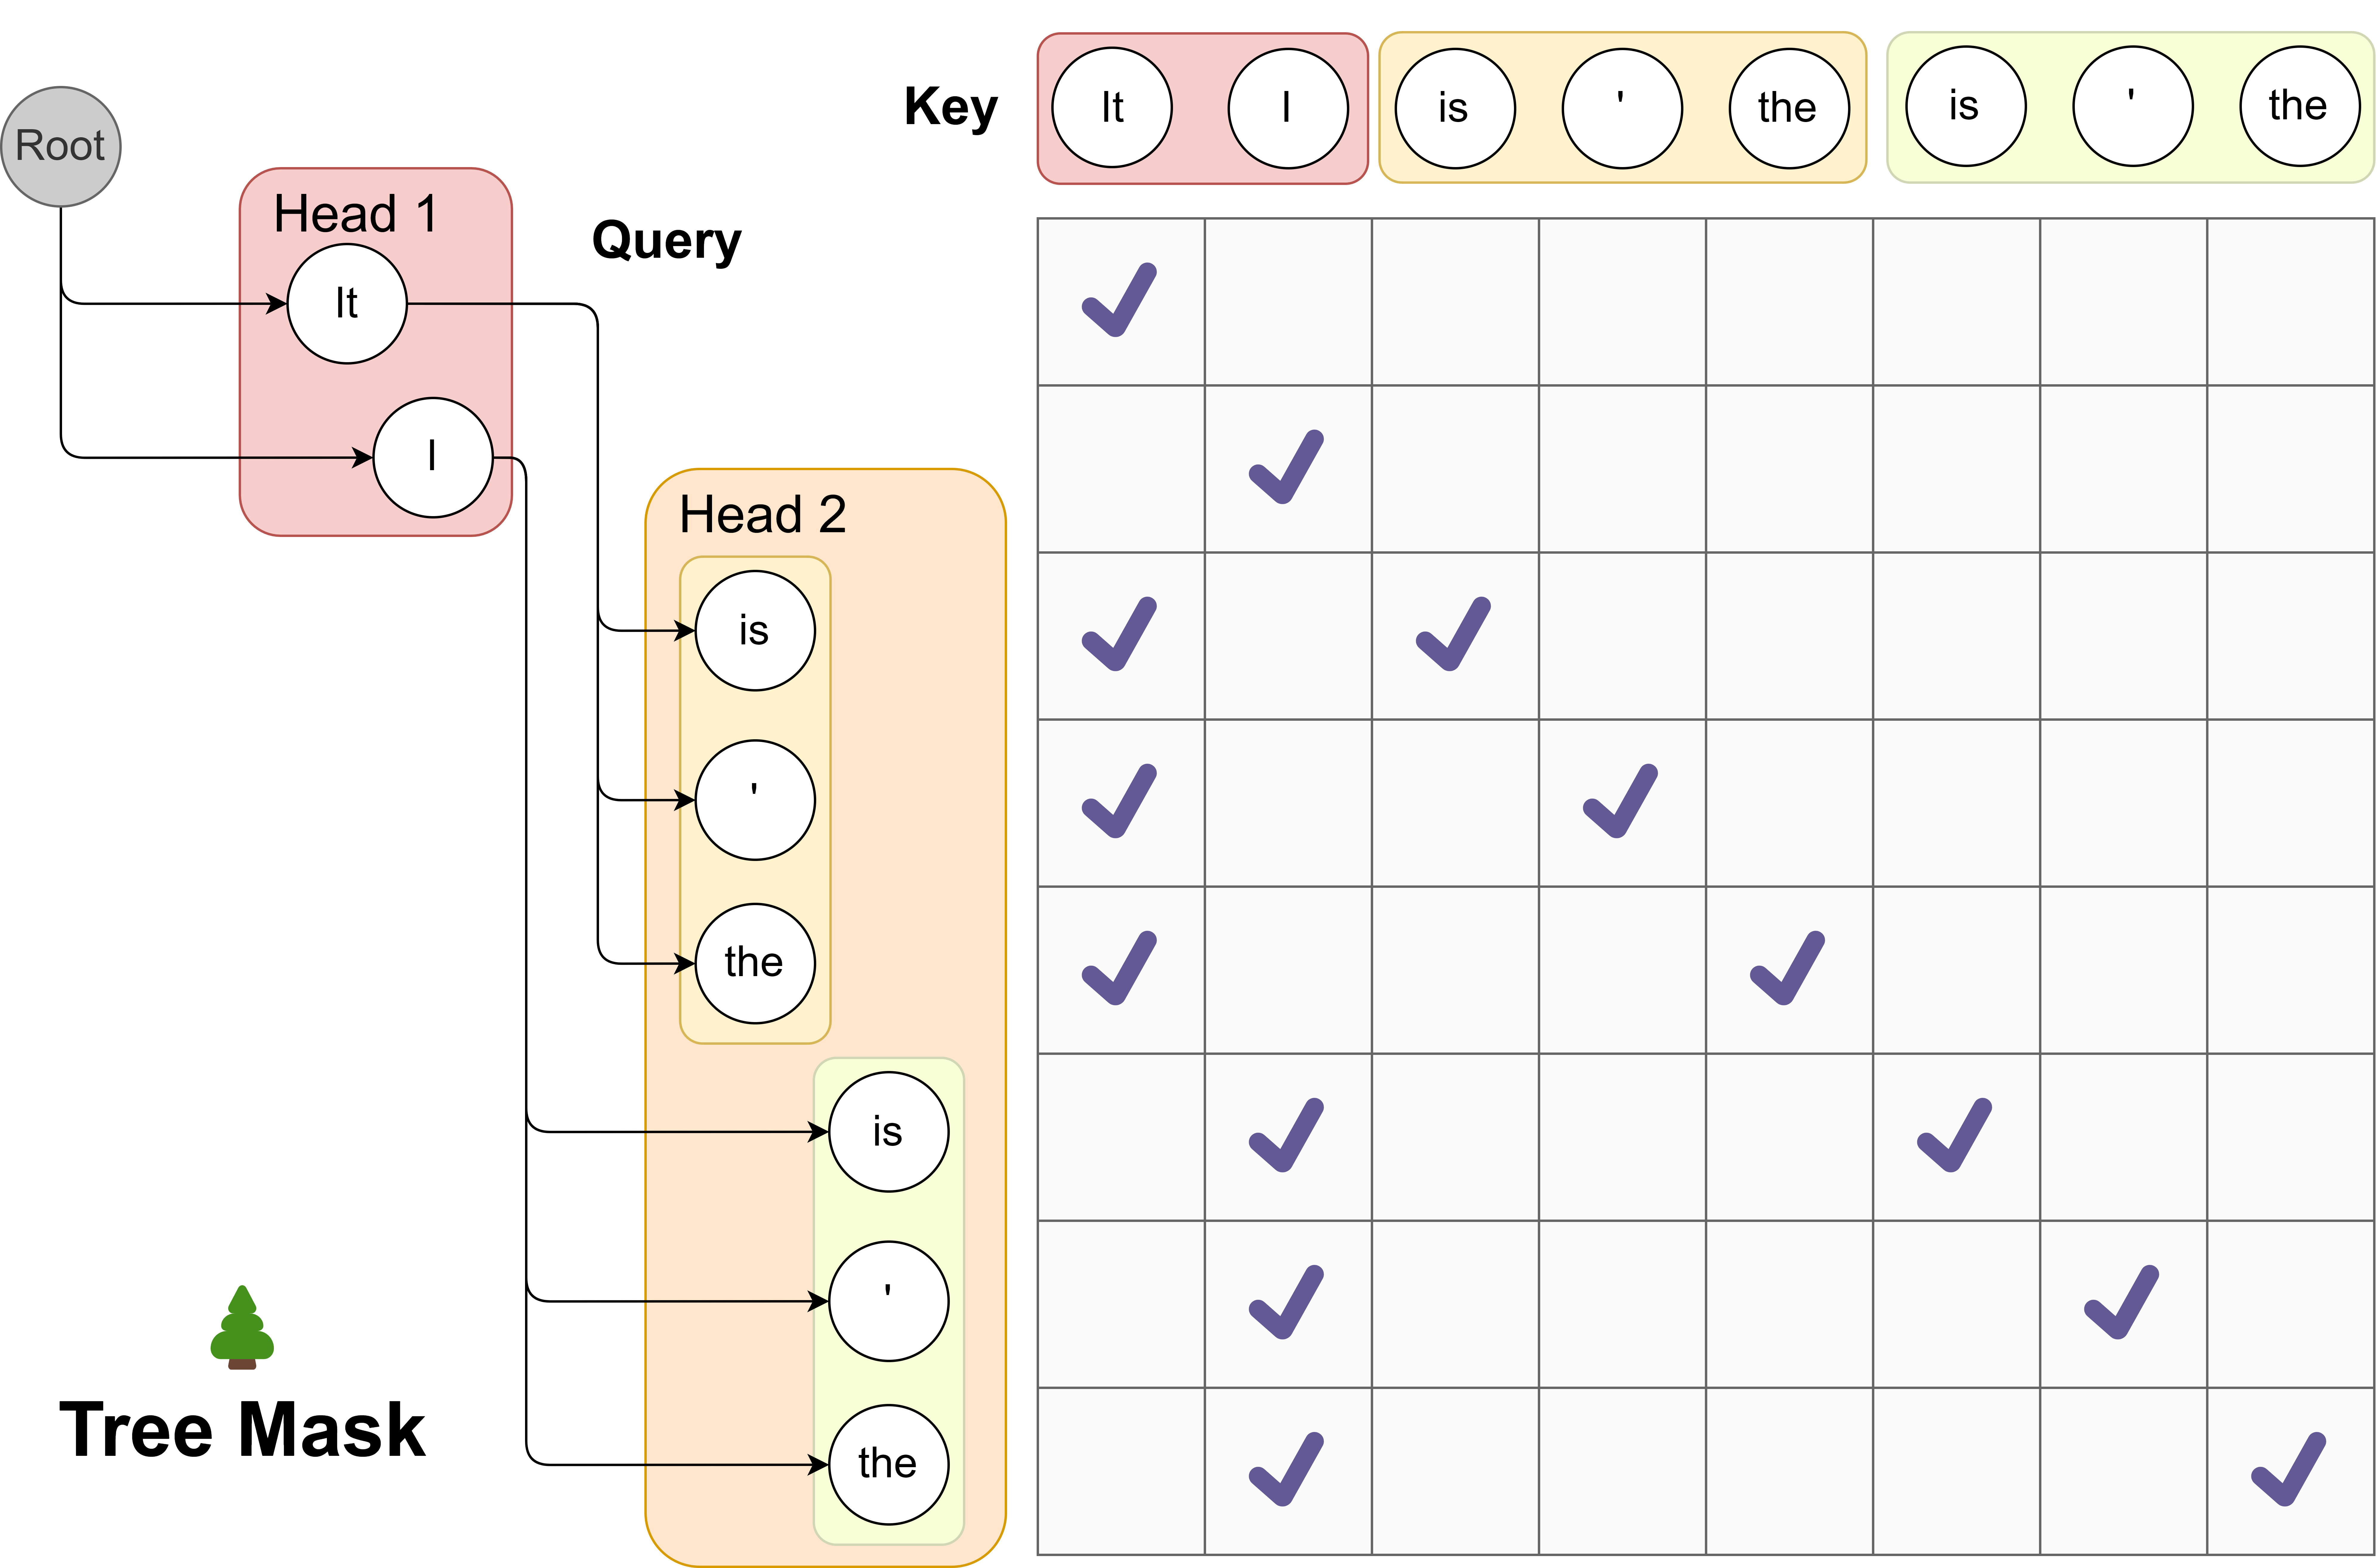
\includegraphics[width=0.45\textwidth]{tree_attention.png}
    \caption{
    We demonstrates the use of tree attention to process multiple candidates concurrently. As exemplified, the top-2 predictions from the first \ours head and the top-3 from the second result in a total of $2\times3=6$ candidates. Each of these candidates corresponds to a distinct branch within the tree structure. To guarantee that each token only accesses its predecessors, we devise an attention mask that exclusively permits attention flow from the current token back to its antecedent tokens. The positional indices for positional encoding are adjusted in line with this structure.}
    \label{fig:tree_attention}
\end{figure}
This attention mechanism diverges from the traditional causal attention paradigm. Within this framework, only tokens from the same continuation are regarded as historical data. Drawing inspiration from the concept of embedding graph structures into attention as proposed in the graph neural network domain~\citep{ying2021transformers}, we incorporate the tree structure into our attention mask, visualized in Figure~\ref{fig:tree_attention}. Remarkably, similar ideas have also been explored in independent works like \citet{miao2023specinfer,spector2023accelerating}, where they follow a bottom-up approach and construct the tree by merging multiple candidates generated by a draft model. In our method, we instead take a top-down approach to build the tree thanks to the structure of candidates generated by \ours heads. For a given $k$-th head, its top-$s_k$ predictions serve as the basis for candidate formation, where $s_k$ is a designated hyperparameter. These candidates are established by determining the Cartesian product of the top-$s_k$ predictions from each head. For instance, in Figure~\ref{fig:tree_attention}, with $s_1=2$ and $s_2=3$, each first head prediction can be succeeded by any prediction from the second head. This leads to a tree structure where $s_k$ branches exist at the $k$-th level (considering a virtual root as the $0$-level, in practice, this $0$-level is for the prediction of the language model head of the original model, which can be sampled independently). Within this tree, only a token's predecessors are seen as historical context, and our attention mask ensures that the attention is only applied on a token's predecessors. By employing this mask and properly setting the positional indices for positional encoding, we can process numerous candidates simultaneously without the need to expand the batch size. The cumulative number of new tokens is calculated as $\sum_{k=1}^K \prod_{i=1}^k s_i$.

In this section, we demonstrate the most simple and regular way to construct the tree structure by taking the Cartesian product. However, it is possible to construct the tree structure in a more sophisticated way and exploit the unbalanced accuracy of different top predictions of different heads. We will discuss this in Section~\ref{sec:optimized_tree_construction}.
\subsection{Training Strategies}
\label{sec:training_recipe}
At the most basic level, we can train \ours heads by freezing the backbone model and fine-tuning \ours heads. However, training the backbone in conjunction with the \ours heads can significantly enhance the accuracy of the \ours heads. Depending on the computational resources and the specific reqirements of the use case, we propose two levels of training strategies for \ours heads.

In this section, we assume the availability of a training dataset that aligns with the target model’s output distribution. This could be the dataset used for Supervised Fine-Tuning (SFT) of the target model. We will discuss eliminating the need for such a dataset using a self-distillation approach in Section~\ref{sec:self_distillation}.
\subsubsection{\ours-1: Frozen Backbone}
\label{sec:frozen_backbone}
To train \ours heads with a frozen backbone model, we can use the cross-entropy loss between the prediction of \ours heads and the ground truth. Specifically, given the ground truth token $y_{t+k+1}$ at position $t+k+1$, the loss for the $k$-th head is $\mathcal{L}_k = -\log p_t^{(k)}(y_{t+k+1})$ where $p_t^{(k)}(y)$ denotes the probability of token $y$ predicted by the $k$-th head. We also observe that $\mathcal{L}_k$ is larger when $k$ is larger, which is reasonable since the prediction of the $k$-th head is more uncertain when $k$ is larger. Therefore, we can add a weight $\lambda_k$ to $\mathcal{L}_k$ to balance the loss of different heads. And the total \ours loss is:
\begin{align}
    \label{eq:loss_medusa_1}
    \mathcal{L}_{\text{\ours-1}} = \sum_{k=1}^K -\lambda_k\log p_t^{(k)}(y_{t+k+1}).
\end{align}

In practice, we set $\lambda_k$ as the $k$-th power of a constant like $0.8$. Since we only use the backbone model for providing the hidden states, we can use a quantized version of the backbone model to reduce the memory consumption. This introduces a more democratized way to accelerate LLM inference, as with the quantization, \ours can be trained for a large model on a single consumer GPU similar to QLoRA~\citep{dettmers2023qlora}. The training only takes a few hours (e.g., 5 hours for \ours-1 on Vicuna 7B model with a single NVIDIA A100 PCIE GPU to train on 60k ShareGPT samples).
\subsubsection{\ours-2: Joint Training}
\label{sec:joint_training}
To further improve the accuracy of \ours heads, we can train \ours heads together with the backbone model. However, this requires a special training recipe to preserve the backbone model's next-token prediction capability and output quality. To achieve this, we propose three strategies:
\begin{itemize}
    \item \textbf{Combined loss}: To keep the backbone model's next-token prediction capability, we need to add the cross-entropy loss of the backbone model $\mathcal{L}_{\text{LM}}=-\log p_t^{(0)}(y_{t+1})$ to the \ours loss. We also add a weight $\lambda_0$ to balance the loss of the backbone model and the \ours heads. Therefore, the total loss is:
    \begin{align}
        \label{eq:loss_medusa_2}
        \mathcal{L}_{\text{\ours-2}} = \mathcal{L}_{\text{LM}} + \lambda_0\mathcal{L}_{\text{\ours-1}}.
    \end{align}
    \item \textbf{Differential learning rates}: Since the backbone model is already well-trained and the \ours heads need more training, we can use separate learning rates for them to enable faster convergence of \ours heads while preserving the backbone model's capability.
    \item \textbf{Heads warmup}: Noticing that at the beginning of training, the \ours heads have a large loss, which leads to a large gradient and may distort the backbone model's parameters. Following the idea from \citet{kumar2022finetuning}, we can employ a two-stage training process. In the first stage, we only train the \ours heads as \ours-1. In the second stage, we train the backbone model and \ours heads together with a warmup strategy. Specifically, we first train the backbone model for a few epochs, then train the \ours heads together with the backbone model. Besides this simple strategy, we can also use a more sophisticated warmup strategy by gradually increasing the weight $\lambda_0$ of the backbone model's loss. We find both strategies work well in practice.
\end{itemize}
Putting these strategies together, we can train \ours heads together with the backbone model without hurting the backbone model's capability. Moreover, this recipe can be applied together with Supervised Fine-Tuning (SFT), enabling us to get a model with native \ours support.
\subsubsection{How to Select the Number of Heads}
Empirically, we found that five heads are sufficient at most. Therefore, we recommend training with five heads and referring to the strategy described in Section~\ref{sec:optimized_tree_construction} to determine the optimal configuration of the tree attention. With optimized tree attention, sometimes three or four heads may be enough for inference. In this case, we can ignore the redundant heads without overhead.

\subsection{Extensions}
\subsubsection{Typical Acceptance}
\label{sec:typical_acceptance}
In speculative decoding papers~\citep{leviathan2022fast,chen2023accelerating}, authors employ rejection sampling to yield diverse outputs that align with the distribution of the original model. However, subsequent implementations~\citep{gante2023assisted,spector2023accelerating} reveal that this sampling strategy results in diminished efficiency as the sampling temperature increases. Intuitively, this can be comprehended in the extreme instance where the draft model is the same as the original one\textcolor{black}{:} 
Using greedy decoding, all output of the draft model will be accepted, therefore maximizing the efficiency. 
Conversely, rejection sampling introduces extra overhead, as the draft model and the original model are sampled independently. Even if their distributions align perfectly, the output of the draft model may still be rejected.

However, in real-world scenarios, sampling from language models is often employed to generate diverse responses, and the temperature parameter is used merely to modulate the ``creativity'' of the response. Therefore, higher temperatures should result in more opportunities for the original model to accept the draft model's output. We ascertain that it is typically unnecessary to match the distribution of the original model. Thus, we propose employing a \emph{typical acceptance} scheme to select plausible candidates rather than using rejection sampling. This approach draws inspiration from truncation sampling studies~\citep{hewitt2022truncation} (refer to \textcolor{black}{Appendix}~\ref{sec:related_work} for an in-depth explanation). Our objective is to choose candidates that are \emph{typical}, meaning they are not exceedingly improbable to be produced by the original model. We use the prediction probability from the \emph{original model} as a natural gauge for this and establish a threshold based on the prediction distribution to determine acceptance. Specifically, given $x_1, x_2, \cdots, x_n$ as context, when evaluating the candidate sequence \textcolor{black}{$(x_{n+1}, x_{n+2}, \cdots, x_{n+K+1})$ }(composed by top predictions of the original language model head and \ours heads), we consider the condition
\begin{align*}
p_{\text{original}}(x_{n+k}|x_1, x_2, \cdots, x_{n+k-1}) > \\\min\rbr{\epsilon, \delta\exp\rbr{-H(p_{\text{original}}(\cdot|x_1, x_2, \cdots, x_{n+k-1}))}},
\end{align*}
where $H(\cdot)$ denotes the entropy function, and $\epsilon, \delta$ are \textcolor{black}{the hard threshold and the entropy-dependent
threshold respectively}. This criterion is adapted from \citet{hewitt2022truncation} and rests on two observations: (1) tokens with relatively high probability are meaningful, and (2) when the distribution's entropy is high, various continuations may be deemed reasonable. During decoding, every candidate is evaluated using this criterion, and a \emph{prefix} of the candidate is accepted if it satisfies the condition. To guarantee the generation of at least one token at each step, we apply \emph{greedy decoding} for the first token and \emph{unconditionally} accept it while employing typical acceptance for subsequent tokens. The final prediction for the current step is determined by the \emph{longest accepted prefix} among all candidates.

Examining this scheme leads to several insights. Firstly, when the temperature is set to $0$, it reverts to greedy decoding, as only the most probable token possesses non-zero probability. As the temperature surpasses $0$, the outcome of greedy decoding will consistently be accepted with appropriate $\epsilon, \delta$, since those tokens have the maximum probability, yielding maximal speedup. Likewise, in general scenarios, an increased temperature will correspondingly result in longer accepted sequences, as corroborated by our experimental findings.

Empirically, we verify that typical acceptance can achieve a better speedup while maintaining a similar \textcolor{black}{generation quality} as shown in Figure~\ref{fig:threshold_ablation}.
\subsubsection{Self-Distillation}
\label{sec:self_distillation}
In Section~\ref{sec:training_recipe}, we assume the existence of a training dataset that matches the target model's output distribution. However, this is not always the case. For example, the model owners may only release the model without the training data, or the model may have gone through a Reinforcement Learning with Human Feedback (RLHF) procedure, which makes the output distribution of the model different from the training dataset. To tackle this issue, we propose an automated self-distillation pipeline to use the model itself to generate the training dataset for \ours heads, which matches the output distribution of the model.

The dataset generation process is straightforward. We first take a public seed dataset from a domain similar to the target model; for example, using the ShareGPT~\citep{sharegpt2023} dataset for chat models. Then, we simply take the prompts from the dataset and ask the model to reply to the prompts. In order to obtain multi-turn conversation samples, we can sequentially feed the prompts from the seed dataset to the model. Or, for models like Zephyr 7B~\citep{tunstall2023zephyr}, which are trained on both roles of the conversation, they have the ability to self-talk, and we can simply feed the first prompt and let the model generate multiple rounds of conversation.

For \ours-1, this dataset is sufficient for training \ours heads. However, for \ours-2, we observe that solely using this dataset for training the backbone and \ours heads usually leads to a lower generation quality. In fact, even without training \ours heads, training the backbone model with this dataset will lead to performance degradation. This suggests that we also need to use the original model's probability prediction instead of using the ground truth token as the label for the backbone model, similar to classic knowledge distillation works~\citep{kim2016sequencelevel}. Concretely, the loss for the backbone model is:
\begin{align*}
    \mathcal{L}_{\text{LM-distill}} = KL(p_{\text{original},t}^{(0)}||p_t^{(0)}),
\end{align*}
where $p_{\text{original},t}^{(0)}$ denotes the probability distribution of the original model's prediction at position $t$.

However, naively, to obtain the original model's probability prediction, we need to maintain two models during training, increasing the memory requirements. To further alleviate this issue, we propose a simple yet effective way to exploit the self-distillation setup. We can use a parameter-efficient adapter like LoRA~\citep{hu2021lora} for fine-tuning the backbone model. In this way, the original model is simply the model with the adapter turned off. Therefore, the distillation does not require additional memory consumption. Together, this self-distillation pipeline can be used to train \ours-2 without hurting the backbone model's capability and introduce almost no additional memory consumption. Lastly, one tip about using self-distillation is that it is preferable to use LoRA without quantization in this case, otherwise, the teacher model will be the quantized model, which may lead to a lower generation quality.

\subsubsection{Searching for the Optimized Tree Construction}
\label{sec:optimized_tree_construction}
In Section~\ref{sec:tree_attention}, we present the simplest way to construct the tree structure by taking the Cartesian product. However, with a fixed budget for the number of total nodes in the tree, a regular tree structure may not be the best choice. Intuitively, those candidates composed of the top predictions of different heads may have different accuracies. Therefore, we can leverage an estimation of the accuracy to construct the tree structure.

Specifically, we can use a calibration dataset and calculate the accuracies of the top predictions of different heads. Let $a_k^{(i)}$ denote the accuracy of the $i$-th top prediction of the $k$-th head\footnote{Here, the accuracy is defined for the single top $i$-th token, i.e., this accuracy is equal to top-$i$ accuracy minus top-$(i-1)$ accuracy.}. Assuming the accuracies are independent, we can estimate the accuracy of a candidate sequence composed by the top $\sbr{i_1, i_2, \cdots, i_k}$ predictions of different heads as $\prod_{j=1}^k a_j^{(i_j)}$. Let $I$ denote the set of all possible combinations of $\sbr{i_1, i_2, \cdots, i_k}$ and each element of $I$ can be mapped to a node of the tree (not only leaf nodes but all nodes are included). Then, the expectation of the acceptance length of a candidate sequence is:
\begin{align*}
    \sum_{\sbr{i_1, i_2, \cdots, i_k}\in I}\prod_{j=1}^k a_j^{(i_j)}.
\end{align*}
Thinking about building a tree by adding nodes one by one, the contribution of a new node to the expectation is exactly the accuracy associated with the node. Therefore, we can greedily add nodes to the tree by choosing the node that is connected to the current tree and has the highest accuracy. This process can be repeated until the total number of nodes reaches the desired number. In this way, we can construct a tree that maximizes the expectation of the acceptance length. Further details can be found in Appendix~\ref{appendix:sparse_tree}.


\section{\hthree Evaluation}
\label{sec:evaluation}

\begin{table}[t]
    % \captionsetup{font=small}
    \small
    \centering
    % \vspace{-1em}
    \caption{\label{table:gpt} Perplexity (lower is better) of models on the Pile, OpenWebText and
      WikiText-103. GPT-Neo and hybrid \hthree are trained on the Pile, while GPT2 is
      trained on WebText. All models use the same GPT2 tokenizer. We report the
      perplexity of GPT-2 models on the Pile ($^*$) for context, though the performance is not directly comparable since they were trained on different data.}
  %   \vspace{1em}
    {
      \begin{tabular}{@{}|c|c|cc|@{}}
      %   \specialrule{.15em}{.05em}{.05em}
      \hline
        Model & Pile & OpenWebText & WikiText103 \\ % & Training time \\
      %   \specialrule{.15em}{.05em}{.05em}
        \hline
        % GPT-2 small (125M) & 9.8 & 18.2 & -- \\ % & 4.7 days \\
        % H3 (126M) & 18.7 & 4.5 days \\ \hline
        % OPT-125M & -- & -- & -- \\
        GPT-2 small (125M) & 19.0* & 22.6 & 29.9 \\
        GPT-Neo-125M & 9.4 & 22.6 & 26.3 \\
        % GPT3-125M (our replication) & - & - & 24.6 \\
        \textbf{Hybrid H3-125M} & \textbf{8.8} & \textbf{20.9} & \textbf{23.7} \\ \hline %2.7 days \\ \hline
        GPT-2 medium (355M) & 13.9* & 17.0 & 21.8 \\ % & 11.5 days \\
        % H3 (361M) &  &  \\ \hline
        % OPT-350M & -- & -- & -- \\
        % GPT3-355M (our replication) & - & - & 16.6 \\
        \textbf{Hybrid H3-355M} & \textbf{7.1} & \textbf{15.9} & \textbf{16.9} \\ \hline
        GPT-2 XL (1.5B) & 12.4* & 12.9 & 17.0 \\
        % OPT-1.3B & -- & -- & -- \\
        GPT-Neo-1.3B & 6.2 & 13.1 & 13.3 \\
        \textbf{Hybrid H3-1.3B} & \textbf{6.0} & \textbf{12.4} & \textbf{12.5} \\
        \hline
        GPT-Neo-2.7B & 5.7 & 11.7 & 11.5 \\
        \textbf{Hybrid H3-2.7B} & \textbf{5.4} & \textbf{11.0} & \textbf{10.6} \\
        \hline
      \end{tabular}
    }
    % \vspace{-1.5em}
  \end{table}

\begin{table}[t]
    % \captionsetup{font=small}
    \scriptsize
    \centering
    % \vspace{-1em}
    \caption{\label{table:superglue_zeroshot_logit} Zero-shot acc.\ on SuperGLUE with logit scoring. Best results in bold, second best underline. }
    %   \vspace{1em}
    {
        \begin{tabular}{@{}|c|cccccccc|c|@{}}
            \hline
        %   \specialrule{.15em}{.05em}{.05em}
        Model & WSC & WIC & RTE & CB & MultiRC & ReCoRD & BoolQ & COPA & Average \\ % & Training time \\
        %   \specialrule{.15em}{.05em}{.05em}
        \hline
        % GPT-2 small (125M) & -- & -- & -- & -- & -- & -- & -- & -- & -- \\ % & 4.7 days \\
        % H3 (126M) & 18.7 & 4.5 days \\ \hline
        OPT-125M & \textbf{39.4} & \underline{52.0} & 48.7 & 37.4 & \underline{58.9} & \underline{44.9} & \underline{59.6} & \underline{60.0} & 50.1 \\
        GPT-Neo-125M & \underline{36.5} & \textbf{53.6} & \underline{53.1} & \underline{41.1} & \textbf{59.9} & 39.6 & \textbf{62.2} & \underline{60.0} & \underline{50.8} \\
        % \textbf{\hthree-125M} & 0.0 & 0.0 & 47.3 & 8.9 & 0.0 & -- & 37.8 & 51.0 & 20.7 \\ %2.7 days \\ \hline
        \textbf{Hybrid \hthree-125M} & \textbf{39.4} & 51.4 & \textbf{59.2} & \textbf{48.2} & 51.4 & \textbf{55.0} & \underline{59.6} & \textbf{67.0} & \textbf{53.9} \\ \hline %2.7 days \\ \hline
        GPT-2 medium (355M) & \underline{50.0} & \textbf{52.0} & 51.3 & 28.6 & \textbf{59.5} & \underline{53.3} & \underline{61.0} & \underline{65.0} & 52.6 \\
        % H3 (361M) &  &  \\ \hline
        OPT-350M & \textbf{53.5} & 50.8 & \underline{53.4} & \underline{35.7} & \underline{58.9} & 51.4 & 60.9 & 60.0 & \underline{53.1} \\
        \textbf{Hybrid \hthree-355M} & 37.5 & \underline{51.7} & \textbf{55.2} & \textbf{41.1} & \textbf{59.5} & \textbf{62.3} & \textbf{61.5} & \textbf{69.0} & \textbf{54.7} \\ \hline
        % GPT-2 (1.5B) & 14.4 & \textbf{36.5} & \underline{49.1} & \underline{8.9} & 0.5 & \underline{44.0} & \underline{46.6} & 59.0 & 32.4 \\
        OPT-1.3B & 36.5 & 49.5 & \textbf{53.4} & \textbf{39.3} & \textbf{58.3} & \underline{61.8} & 55.0 & \underline{69.0} & \underline{52.9} \\
        GPT-Neo-1.3B & \underline{41.3} & \underline{50.0} & \underline{52.3} & \underline{33.9} & 57.9 & 55.5 & \underline{59.9} & 66.0 & 52.1 \\
        \textbf{Hybrid \hthree-1.3B} & \textbf{52.9} & \textbf{50.3} & \textbf{53.4} & \underline{33.9} & \underline{58.2} & \textbf{67.8} & \textbf{61.7} & \textbf{74.0} & \textbf{56.5} \\ \hline
        OPT-2.7B & \textbf{51.0} & \underline{50.8} & 50.5 & \underline{41.1} & 57.4 & \underline{65.9} & 60.9 & 66.0 & \underline{55.5} \\
        GPT-Neo-2.7B & \underline{37.5} & 50.0 & \underline{52.3} & \textbf{50.0} & \textbf{59.1} & 60.0 & \textbf{61.1} & \underline{67.0} & 54.6 \\
        \textbf{Hybrid \hthree-2.7B} & 36.5 & \textbf{51.3} & \textbf{57.0} & 37.5 & \underline{58.7} & \textbf{71.3} & \textbf{61.1} & \textbf{81.0} & \textbf{56.8} \\ \hline
        \end{tabular}
    }
    % \vspace{-1.5em}
\end{table}
\begin{table}[t]
    % \captionsetup{font=small}
    \scriptsize
    \centering
    % \vspace{-1em}
    \caption{\label{table:superglue_fewshot_logit} 3-shot acc.\ on SuperGLUE with logit scoring. Best results in bold, second best underline. }
    %   \vspace{1em}
    {
        \begin{tabular}{@{}|c|cccccccc|c|@{}}
            \hline
        %   \specialrule{.15em}{.05em}{.05em}
        Model & WSC & WIC & RTE & CB & MultiRC & ReCoRD & BoolQ & COPA & Average \\ % & Training time \\
        %   \specialrule{.15em}{.05em}{.05em}
        \hline
        % GPT-2 small (125M) & -- & -- & -- & -- & -- & -- & -- & -- & -- \\ % & 4.7 days \\
        % H3 (126M) & 18.7 & 4.5 days \\ \hline
        OPT-125M & 36.5 & \textbf{50.2} & 47.3 & \underline{44.6} & \textbf{57.9} & \underline{44.9} & 41.9 & 60.0 & \underline{47.9} \\
        GPT-Neo-125M & \underline{38.5} & \underline{50.0} & \underline{53.1} & 17.9 & \underline{56.3} & 39.6 & \textbf{62.1} & \underline{60.0} & 47.2 \\
        \textbf{Hybrid \hthree-125M} & \textbf{43.3} & 49.1 & \textbf{58.1} & \textbf{51.8} & 48.9 & \textbf{55.0} & \underline{56.1} & \textbf{67.0} & \textbf{53.7} \\ \hline %2.7 days \\ \hline
        GPT-2 medium (355M) & 36.5 & \textbf{50.5} & \underline{48.0} & 8.9 & 43.5 & \underline{53.3} & 58.8 & \underline{65.0} & 45.6 \\
        % H3 (361M) &  &  \\ \hline
        OPT-350M & \underline{37.5} & \underline{50.0} & 45.8 & \textbf{44.6} & \underline{49.8} & 51.4 & \textbf{61.7} & 60.0 & \underline{50.1} \\
        \textbf{Hybrid \hthree-355M} & \textbf{42.3} & 47.5 & \textbf{50.5} & \underline{28.6} & \textbf{59.7} & \textbf{62.3} & \underline{60.5} & \textbf{69.0} & \textbf{52.6} \\ \hline
        % GPT-2 (1.5B) & \underline{36.5} & 36.5 & \textbf{56.7} & 41.1 & 6.1 & 43.8 & \underline{53.7} & 61.0 & 41.9 \\
        OPT-1.3B & \textbf{44.2} & \textbf{51.1} & \underline{53.4} & 16.1 & \textbf{59.9} & \underline{62.1} & 38.3 & \underline{70.0} & 49.4 \\
        GPT-Neo-1.3B & 35.6 & \underline{50.6} & 47.3 & \textbf{32.1} & \textbf{59.9} & 55.7 & \textbf{61.2} & 67.0 & \underline{51.2} \\
        \textbf{Hybrid \hthree-1.3B} & \underline{36.5} & 49.2 & \textbf{55.2} & \underline{23.2} & \underline{59.3} & \textbf{67.6} & \underline{56.9} & \textbf{76.0} & \textbf{53.0} \\ \hline
        OPT-2.7B & \underline{44.2} & \underline{50.5} & \textbf{53.4} & 17.9 & \underline{59.2} & \underline{66.0} & \textbf{62.0} & \underline{71.0} & \underline{53.0} \\
        GPT-Neo-2.7B & \textbf{49.0} & \textbf{51.9} & \underline{51.6} & \underline{21.4} & 57.0 & 60.0 & 56.0 & 68.0 & 51.9 \\
        \textbf{Hybrid \hthree-2.7B} & 36.5 & 45.6 & 47.3 & \textbf{46.4} & \textbf{59.4} & \textbf{71.1} & \underline{60.6} & \textbf{77.0} & \textbf{55.5} \\ \hline
        \end{tabular}
    }
    % \vspace{-1.5em}
\end{table}

To understand how well capturing the synthetics in Section~\ref{sec:synthetics} translates to language modeling, we train two hybrid hybrid \hthree-attention language models at sizes 125M, 355M, 1.3B, and 2.7B, and we evaluate their performance against Transformers.
The hybrid models match or exceed the quality of Transformers in perplexity and zero/few-shot learning.
We also validate that \hthree models retain strong performance on non-text sequence modeling.
Appendix~\ref{sec:app_additional_experiments} contains additional experiments on more datasets, length extrapolation, and scaling with data.

\subsection{Language Modeling}
\label{subsec:language_modeling}

We compare hybrid \hthree-attention language models against Transformer-based language models.
We evaluate language modeling performance using perplexity, zero-shot learning, and few-shot learning performance.
Hybrid \hthree models outperform Transformers, which suggests that closing the gap between SSMs and attention on the synthetic languages translates to real language modeling capabilities.
We also report the generation speed of hybrid \hthree models compared to Transformers; since SSMs are recurrent models, they can generate tokens \num{2.4$\times$} faster than Transformers.
Appendix~\ref{sec:app_additional_experiments} shows performance of pure \hthree language models on these same evaluation metrics.

\paragraph{Setup}
We train hybrid models at sizes 125M, 355M, 1.3B, and 2.7B on the Pile~\citep{gao2020pile} for 400B tokens.
We compare against checkpoints of equivalent sizes from
Open-AI~\citep{radford2019language} and GPT-Neo\footnote{There
  is no pretrained GPT-Neo at the 350M size.}~\citep{gpt-neo},
from HuggingFace~\citep{wolf-etal-2020-transformers}.


\paragraph{Perplexity}
Table \ref{table:gpt} shows perplexity on the Pile~\citep{gao2020pile}, OpenWebText~\citep{Gokaslan2019OpenWeb}, and WikiText-103~\citep{merity2016pointer}. 
On the Pile, our 125M hybrid model outperforms GPT-Neo, which was also trained on the Pile.
Our hybrid models also outperform GPT-Neo models and GPT-2 models on zero-shot transfer to OpenWebText and WikiText103.
We report the PPL of GPT-2 models for context, though the performance is not directly comparable since they were trained on different data.

\paragraph{Zero- and Few-shot Performance}
We compare the zero- and few-shot performance of hybrid \hthree language models against OPT~\citep{zhang2022opt}, GPT-Neo, and GPT-2 models, where public checkpoints are available.
We report performance with rank classification on the logits of the possible choices (see Appendix~\ref{sec:app_generation} for raw generation).
Table~\ref{table:superglue_zeroshot_logit} reports zero-shot performance on the SuperGLUE benchmark, and Table~\ref{table:superglue_fewshot_logit} reports the 3-shot performance.
Following the perplexity results, the hybrid language models outperform or match the best the Transformer baseline on more than half the tasks.

\begin{table}[t]
\centering
% \begin{table}[h]
    % \captionsetup{font=small}
    \small
    \centering
    % \vspace{-1em}
    \caption{\label{table:training_time} Inference throughput on A100 80GB, 1.3B models.
    Batch size 64, prompt length 512, 1024, or 1536, and generating 128 tokens
    per sequence in the batch (i.e., 64 $\times$ 128 tokens in a batch). Hybrid
    \hthree is up to 2.4$\times$ faster than a Transformer of similar size in inference. The
    difference is larger for longer sequences.}
    %   \vspace{1em}
    {
        \begin{tabular}{@{}|c|c|c|c|@{}}
            \hline
        %   \specialrule{.15em}{.05em}{.05em}
        Tokens/s & Prompt length 512 & Prompt length 1024 & Prompt length 1536 \\ % & Training time \\
        %   \specialrule{.15em}{.05em}{.05em}
        \hline
        Transformer-1.3B & 1340 & 770 & 520 \\
        % GPT-2 Small (FlashAttention~\citep{dao2022flashattention}) & -- & -- \\ 
        % GPT-2 Small (FasterTransformer~\citep{}) & N/A & -- \\ \hline
        Hybrid \hthree-1.3B & 1980 & 1580 & 1240 \\ \hline
        \end{tabular}
    }
    % \vspace{-1.5em}
% \end{table}
\end{table}
\paragraph{Language Modeling Inference}
Finally, since SSMs are recurrent models, they admit faster text generation than Transformers.
Table~\ref{table:training_time} shows inference throughput of a 1.3B-parameter hybrid model compared to a Transformer.
The hybrid model has up to \num{2.4$\times$} higher throughput.



%%% Local Variables:
%%% mode: latex
%%% TeX-master: "../main"
%%% End:

\section{\fastfft Evaluation \label{sec:eval_efficiency}}
We evaluate how well \fastfft speeds up SSMs.
\fastfft sets state-of-the-art performance on the long range arena benchmark~\citep{tay2020long} using S4~\citep{gu2022efficiently}.
We report performance of training \hthree module with \fastfft compared to attention at various sequence lengths, from 256 to 32K and demonstrate nearly linear scaling.

\begin{table}[t]
    \centering
    % \begin{table}[h]
%   \vspace{-1em}
    \caption{\label{table:lra} Speedup on the LRA benchmark.}
    \centering
    \small
    % \setlength{\tabcolsep}{10pt}
    % \renewcommand{\arraystretch}{1.1}
%   \iftoggle{arxiv}{}{
%     \resizebox{0.9\linewidth}{!}
%   }
%   {
    \begin{tabular}{|c|c|}
    %   \specialrule{.15em}{.05em}{.05em}
    %   \multirow{1}{*}{ {\bf Model} }  &
    %   \multicolumn{1}{c}{\multirow{1}{*}{ListOps}} &
    %   \multicolumn{1}{c}{\multirow{1}{*}{Text}} &
    %   \multicolumn{1}{c}{\multirow{1}{*}{Retrieval}} &
    %   \multicolumn{1}{c}{\multirow{1}{*}{Image}} &
    %   \multicolumn{1}{c|}{\multirow{1}{*}{Pathfinder}}  &
    %   \multicolumn{1}{c|}{\multirow{1}{*}{Avg}} &
    %   \multicolumn{1}{c|}{\multirow{1}{*}{Speedup}}
    %   % \multicolumn{1}{c}{\multirow{1}{*}{Mem.\ saving}}
    %   \\
    \hline
    Models &  Speedup \\
    \hline
    Transformer & 1$\times$  \\
    FlashAttention~\citep{dao2022flashattention} & 2.4$\times$ \\
    Block-sparse FlashAttention~\citep{dao2022flashattention} & 2.8$\times$ \\
    % Linformer~\citep{wang2020linformer} & 2.5$\times$ \\
    % Linear Attention~\citep{katharopoulos2020transformers} & 2.3$\times$ \\
    % Performer~\citep{choromanski2020rethinking} & 1.8$\times$ \\
    % Local Attention~\citep{tay2020long} & 1.7$\times$ \\
    % Reformer~\citep{kitaev2020reformer} & 1.3$\times$  \\
    % Smyrf~\citep{daras2020smyrf} & 1.7$\times$ \\
    \hline
%   MEGA \\
    S4~\citep{gu2022train} & 2.9$\times$ \\
%   H3 (maybe?) \\
    S4 with \fastfft & \num{5.8$\times$} \\ \hline
    % \specialrule{.15em}{.05em}{.05em}
    \end{tabular}
%   }
    % \vspace{-1em}
% \end{table}

% \begin{table}[h]
%     %   \vspace{-1em}
%         \caption{\label{table:lra} Performance on the Long-Range-Arena benchmarks.}
%         \centering
%         \small
%         % \setlength{\tabcolsep}{10pt}
%         % \renewcommand{\arraystretch}{1.1}
%     %   \iftoggle{arxiv}{}{
%     %     \resizebox{0.9\linewidth}{!}
%     %   }
%     %   {
%         \begin{tabular}{|c|ccccc|c|c|c|}
%       %   \specialrule{.15em}{.05em}{.05em}
%       %   \multirow{1}{*}{ {\bf Model} }  &
%       %   \multicolumn{1}{c}{\multirow{1}{*}{ListOps}} &
%       %   \multicolumn{1}{c}{\multirow{1}{*}{Text}} &
%       %   \multicolumn{1}{c}{\multirow{1}{*}{Retrieval}} &
%       %   \multicolumn{1}{c}{\multirow{1}{*}{Image}} &
%       %   \multicolumn{1}{c|}{\multirow{1}{*}{Pathfinder}}  &
%       %   \multicolumn{1}{c|}{\multirow{1}{*}{Avg}} &
%       %   \multicolumn{1}{c|}{\multirow{1}{*}{Speedup}}
%       %   % \multicolumn{1}{c}{\multirow{1}{*}{Mem.\ saving}}
%       %   \\
%         \hline
%       Models & ListOps & Text & Retrieval & Image & Pathfinder & Avg & Path-X &  Speedup \\
%         \hline
%         Transformer & 36.0 & 63.6 & 81.6 & 42.3 & 72.7 & 59.3 & x & 1$\times$  \\
%       FlashAttention & 37.6 & 63.9 & 81.4 & 43.5 & 72.7 & 59.8 & 61.4 & 2.4$\times$ \\
%       Block-sparse FlashAttention & 37.0 & 63.0 & 81.3 & 43.6 & 73.3 & 59.6 & 56.0 & 2.8$\times$ \\
%       Linformer~\citep{wang2020linformer} & 35.6 & 55.9 & 77.7 & 37.8 & 67.6 & 54.9 & x & 2.5$\times$ \\
%       Linear Attention~\citep{katharopoulos2020transformers} & 38.8 & 63.2 & 80.7 & 42.6 & 72.5 & 59.6 & x & 2.3$\times$ \\
%       Performer~\citep{choromanski2020rethinking} & 36.8 & 63.6 & 82.2 & 42.1 & 69.9 & 58.9 & x & 1.8$\times$ \\
%       Local Attention~\citep{tay2020long} & 36.1 & 60.2 & 76.7 & 40.6 & 66.6 & 56.0 & x & 1.7$\times$ \\
%       Reformer~\citep{kitaev2020reformer} & 36.5 & 63.8 & 78.5 & 39.6 & 69.4 & 57.6 & x & 1.3$\times$  \\
%       Smyrf~\citep{daras2020smyrf} & 36.1 & 64.1 & 79.0 & 39.6 & 70.5 & 57.9 & x & 1.7$\times$ \\
%       \cline{1-8}
%       \hline
%     %   MEGA \\
%       S4~\citep{gu2022train} & 59.6 & 86.8 & 90.9 & 88.7 & 94.2 & 84.0 & 96.4 & 2.9$\times$ \\
%     %   H3 (maybe?) \\
%       S4 with \fastfft & 59.6 & 86.8 & 90.9 & 88.7 & 94.2 & 84.0 & 96.4 & -- \\ \hline
%         % \specialrule{.15em}{.05em}{.05em}
%         \end{tabular}
%     %   }
%         \label{table:lra}
%         % \vspace{-1em}
%     \end{table}
\end{table}

\paragraph{Long Range Arena}
The Long Range Arena (LRA) benchmark~\citep{tay2020long} is a benchmark for long-range sequence modeling.
The state-of-the-art approach, S4~\citep{gu2022train}, is an SSM.
Table~\ref{table:lra} shows that \fastfft accelerates S4 by 2$\times$, outperforming Transformers by 5.8$\times$.

\section{\fastfft Evaluation \label{sec:eval_efficiency}}
We evaluate how well \fastfft speeds up SSMs.
\fastfft sets state-of-the-art performance on the long range arena benchmark~\citep{tay2020long} using S4~\citep{gu2022efficiently}.
We report performance of training \hthree module with \fastfft compared to attention at various sequence lengths, from 256 to 32K and demonstrate nearly linear scaling.

\begin{table}[t]
    \centering
    % \begin{table}[h]
%   \vspace{-1em}
    \caption{\label{table:lra} Speedup on the LRA benchmark.}
    \centering
    \small
    % \setlength{\tabcolsep}{10pt}
    % \renewcommand{\arraystretch}{1.1}
%   \iftoggle{arxiv}{}{
%     \resizebox{0.9\linewidth}{!}
%   }
%   {
    \begin{tabular}{|c|c|}
    %   \specialrule{.15em}{.05em}{.05em}
    %   \multirow{1}{*}{ {\bf Model} }  &
    %   \multicolumn{1}{c}{\multirow{1}{*}{ListOps}} &
    %   \multicolumn{1}{c}{\multirow{1}{*}{Text}} &
    %   \multicolumn{1}{c}{\multirow{1}{*}{Retrieval}} &
    %   \multicolumn{1}{c}{\multirow{1}{*}{Image}} &
    %   \multicolumn{1}{c|}{\multirow{1}{*}{Pathfinder}}  &
    %   \multicolumn{1}{c|}{\multirow{1}{*}{Avg}} &
    %   \multicolumn{1}{c|}{\multirow{1}{*}{Speedup}}
    %   % \multicolumn{1}{c}{\multirow{1}{*}{Mem.\ saving}}
    %   \\
    \hline
    Models &  Speedup \\
    \hline
    Transformer & 1$\times$  \\
    FlashAttention~\citep{dao2022flashattention} & 2.4$\times$ \\
    Block-sparse FlashAttention~\citep{dao2022flashattention} & 2.8$\times$ \\
    % Linformer~\citep{wang2020linformer} & 2.5$\times$ \\
    % Linear Attention~\citep{katharopoulos2020transformers} & 2.3$\times$ \\
    % Performer~\citep{choromanski2020rethinking} & 1.8$\times$ \\
    % Local Attention~\citep{tay2020long} & 1.7$\times$ \\
    % Reformer~\citep{kitaev2020reformer} & 1.3$\times$  \\
    % Smyrf~\citep{daras2020smyrf} & 1.7$\times$ \\
    \hline
%   MEGA \\
    S4~\citep{gu2022train} & 2.9$\times$ \\
%   H3 (maybe?) \\
    S4 with \fastfft & \num{5.8$\times$} \\ \hline
    % \specialrule{.15em}{.05em}{.05em}
    \end{tabular}
%   }
    % \vspace{-1em}
% \end{table}

% \begin{table}[h]
%     %   \vspace{-1em}
%         \caption{\label{table:lra} Performance on the Long-Range-Arena benchmarks.}
%         \centering
%         \small
%         % \setlength{\tabcolsep}{10pt}
%         % \renewcommand{\arraystretch}{1.1}
%     %   \iftoggle{arxiv}{}{
%     %     \resizebox{0.9\linewidth}{!}
%     %   }
%     %   {
%         \begin{tabular}{|c|ccccc|c|c|c|}
%       %   \specialrule{.15em}{.05em}{.05em}
%       %   \multirow{1}{*}{ {\bf Model} }  &
%       %   \multicolumn{1}{c}{\multirow{1}{*}{ListOps}} &
%       %   \multicolumn{1}{c}{\multirow{1}{*}{Text}} &
%       %   \multicolumn{1}{c}{\multirow{1}{*}{Retrieval}} &
%       %   \multicolumn{1}{c}{\multirow{1}{*}{Image}} &
%       %   \multicolumn{1}{c|}{\multirow{1}{*}{Pathfinder}}  &
%       %   \multicolumn{1}{c|}{\multirow{1}{*}{Avg}} &
%       %   \multicolumn{1}{c|}{\multirow{1}{*}{Speedup}}
%       %   % \multicolumn{1}{c}{\multirow{1}{*}{Mem.\ saving}}
%       %   \\
%         \hline
%       Models & ListOps & Text & Retrieval & Image & Pathfinder & Avg & Path-X &  Speedup \\
%         \hline
%         Transformer & 36.0 & 63.6 & 81.6 & 42.3 & 72.7 & 59.3 & x & 1$\times$  \\
%       FlashAttention & 37.6 & 63.9 & 81.4 & 43.5 & 72.7 & 59.8 & 61.4 & 2.4$\times$ \\
%       Block-sparse FlashAttention & 37.0 & 63.0 & 81.3 & 43.6 & 73.3 & 59.6 & 56.0 & 2.8$\times$ \\
%       Linformer~\citep{wang2020linformer} & 35.6 & 55.9 & 77.7 & 37.8 & 67.6 & 54.9 & x & 2.5$\times$ \\
%       Linear Attention~\citep{katharopoulos2020transformers} & 38.8 & 63.2 & 80.7 & 42.6 & 72.5 & 59.6 & x & 2.3$\times$ \\
%       Performer~\citep{choromanski2020rethinking} & 36.8 & 63.6 & 82.2 & 42.1 & 69.9 & 58.9 & x & 1.8$\times$ \\
%       Local Attention~\citep{tay2020long} & 36.1 & 60.2 & 76.7 & 40.6 & 66.6 & 56.0 & x & 1.7$\times$ \\
%       Reformer~\citep{kitaev2020reformer} & 36.5 & 63.8 & 78.5 & 39.6 & 69.4 & 57.6 & x & 1.3$\times$  \\
%       Smyrf~\citep{daras2020smyrf} & 36.1 & 64.1 & 79.0 & 39.6 & 70.5 & 57.9 & x & 1.7$\times$ \\
%       \cline{1-8}
%       \hline
%     %   MEGA \\
%       S4~\citep{gu2022train} & 59.6 & 86.8 & 90.9 & 88.7 & 94.2 & 84.0 & 96.4 & 2.9$\times$ \\
%     %   H3 (maybe?) \\
%       S4 with \fastfft & 59.6 & 86.8 & 90.9 & 88.7 & 94.2 & 84.0 & 96.4 & -- \\ \hline
%         % \specialrule{.15em}{.05em}{.05em}
%         \end{tabular}
%     %   }
%         \label{table:lra}
%         % \vspace{-1em}
%     \end{table}
\end{table}

\paragraph{Long Range Arena}
The Long Range Arena (LRA) benchmark~\citep{tay2020long} is a benchmark for long-range sequence modeling.
The state-of-the-art approach, S4~\citep{gu2022train}, is an SSM.
Table~\ref{table:lra} shows that \fastfft accelerates S4 by 2$\times$, outperforming Transformers by 5.8$\times$.

\section{\fastfft Evaluation \label{sec:eval_efficiency}}
We evaluate how well \fastfft speeds up SSMs.
\fastfft sets state-of-the-art performance on the long range arena benchmark~\citep{tay2020long} using S4~\citep{gu2022efficiently}.
We report performance of training \hthree module with \fastfft compared to attention at various sequence lengths, from 256 to 32K and demonstrate nearly linear scaling.

\begin{table}[t]
    \centering
    \input{tables/lra}
\end{table}

\paragraph{Long Range Arena}
The Long Range Arena (LRA) benchmark~\citep{tay2020long} is a benchmark for long-range sequence modeling.
The state-of-the-art approach, S4~\citep{gu2022train}, is an SSM.
Table~\ref{table:lra} shows that \fastfft accelerates S4 by 2$\times$, outperforming Transformers by 5.8$\times$.

\input{figs/efficiency.tex}
\paragraph{Benchmark \hthree Against Attention}
We benchmark the time to run the forward and backward pass of \hthree with \fastfft against attention.
\fastfft maintains nearly linear scaling, even to very long sequence lengths.
\cref{fig:fftconv_speed} shows overall 2-3$\times$ speedup over FFTConv with cuFFT using our techniques
(block FFT, state-passing).
Simple kernel fusion (even without block FFT) can yield speedup over cuFFT for short sequences, since memory reads/writes are the bottleneck for short sequences.
For long sequences, SSMs using state passing can be dozens of times faster
than even the fastest attention implementation.

%%% Local Variables:
%%% mode: latex
%%% TeX-master: "../main"
%%% End:

\paragraph{Benchmark \hthree Against Attention}
We benchmark the time to run the forward and backward pass of \hthree with \fastfft against attention.
\fastfft maintains nearly linear scaling, even to very long sequence lengths.
\cref{fig:fftconv_speed} shows overall 2-3$\times$ speedup over FFTConv with cuFFT using our techniques
(block FFT, state-passing).
Simple kernel fusion (even without block FFT) can yield speedup over cuFFT for short sequences, since memory reads/writes are the bottleneck for short sequences.
For long sequences, SSMs using state passing can be dozens of times faster
than even the fastest attention implementation.

%%% Local Variables:
%%% mode: latex
%%% TeX-master: "../main"
%%% End:

\paragraph{Benchmark \hthree Against Attention}
We benchmark the time to run the forward and backward pass of \hthree with \fastfft against attention.
\fastfft maintains nearly linear scaling, even to very long sequence lengths.
\cref{fig:fftconv_speed} shows overall 2-3$\times$ speedup over FFTConv with cuFFT using our techniques
(block FFT, state-passing).
Simple kernel fusion (even without block FFT) can yield speedup over cuFFT for short sequences, since memory reads/writes are the bottleneck for short sequences.
For long sequences, SSMs using state passing can be dozens of times faster
than even the fastest attention implementation.

%%% Local Variables:
%%% mode: latex
%%% TeX-master: "../main"
%%% End:

%!TEX root = ../main.tex

\section{Conclusion}
\label{sec:conc}

Our main goal is to understand and narrow the gap between attention and SSMs in
language modeling in terms of modeling capabilities and hardware efficiency.
Our exploration based on synthetic language tasks motivated us to design the
\hthree layer, which is surprisingly competitive with attention.
Our \textsc{BlockFFTConv} algorithm exploits matrix multiplication units and the
dual recurrent--convolution view of SSMs to substantially speed up SSMs, reducing
the hardware barrier between attention and SSMs.
We are excited about several future directions.
Our \hthree layer is a simple combination of two SSMs, and more
sophisticated designs could be more expressive.
Our encouraging results on language models up to 1.3B parameters suggests that
scaling SSMs to larger sizes is a promising avenue.
Since simply adding two attention layers to \hthree models already
outperforms both the pure \hthree model and Transformers, we are optimistic
about combining the complementary strengths of SSMs and attention in the future.

% \pagebreak
\ifarxiv

\else
\textbf{Reproducibility Statement.} To facilitate the reproducibility of our
algorithms and results, (i) we include a link to downloadable source code in
supplementary materials, (ii) for our theoretical statements and results, we
include clear explanations of any assumptions and a complete proof of the claims
in~\cref{sec:proofs}; for any datasets used in the experiments, a complete description of the data processing steps is in~\cref{sec:app_exp_details}.
We will also release model checkpoints for all our models.

\textbf{Ethics Statement.}
Our work seeks to understand the fundamental capabilities and limitations of newly-emerging model architectures.
As the amount of data and model size grows, we also week to understand how to make training these models more efficient---and run inference more efficiently.
This potentially connects to energy savings during model development and deployment.
We also note that the relative underutilization of tensor cores in the FFT convolutions of state space models (even with our block FFT) suggests that consumer GPUs may be able to train models at a cheaper price point.

However, as with any language model training, developing new techniques may impact a wide range of applications, each with potential benefits and harms.
For example, making language model training cheaper and making inference more efficient make it cheaper to spread disinformation.
Similarly, improving the efficiency of model training may not reduce the overall environmental footprint of training, since the same resources may be used to train more models, or train the same models for longer.
While our work makes partial progress on the fronts of efficiency and understanding, it does not explicitly address the issues of fairness and bias in language models.
\fi
%%% Local Variables:
%%% mode: latex
%%% TeX-master: "../main"
%%% End:


\section*{Acknowledgments}

We thank Albert Gu for helpful discussion regarding the model architecture, and
more importantly for sending us daily hippo videos.
We thank Together Computer
for providing portions of the compute used to train models in this paper.
We gratefully acknowledge the support of NIH under No. U54EB020405 (Mobilize), NSF under Nos. CCF1763315 (Beyond Sparsity), CCF1563078 (Volume to Velocity), and 1937301 (RTML); ARL under No. W911NF-21-2-0251 (Interactive Human-AI Teaming); ONR under No. N000141712266 (Unifying Weak Supervision); ONR N00014-20-1-2480: Understanding and Applying Non-Euclidean Geometry in Machine Learning; N000142012275 (NEPTUNE); NXP, Xilinx, LETI-CEA, Intel, IBM, Microsoft, NEC, Toshiba, TSMC, ARM, Hitachi, BASF, Accenture, Ericsson, Qualcomm, Analog Devices, Google Cloud, Salesforce, Total, the HAI-GCP Cloud Credits for Research program,  the Stanford Data Science Initiative (SDSI),
Department of Defense (DoD) through the National Defense Science and
Engineering Graduate Fellowship (NDSEG) Program, 
Wu Tsai Neuroscience Stanford Interdisciplinary Graduate Fellowship,
and members of the Stanford DAWN project: Facebook, Google, and VMWare. The U.S. Government is authorized to reproduce and distribute reprints for Governmental purposes notwithstanding any copyright notation thereon. Any opinions, findings, and conclusions or recommendations expressed in this material are those of the authors and do not necessarily reflect the views, policies, or endorsements, either expressed or implied, of DARPA, NIH, ONR, or the U.S. Government.
Atri Rudra’s research is supported by NSF grant CCF-1763481.


\ifarxiv
\bibliographystyle{plain} % arxiv
\else
\bibliographystyle{iclr2023_conference}
\fi
\bibliography{main}

\appendix
\newpage
\section{Related work}

There is a rich prior literature on 
probabilistic programming languages (PPLs),
which extend probabilistic graphical models to
support more complex joint distributions whose size and ``shape''
can itself be stochastic (e.g., a graph
unrolled for a random number of iterations,
until a data-dependent stopping criterion is met).
PPLs extend traditional programming languages with the ability to {\it sample} from distributions and {\it observe} values of variables based on data (i.e. condition the model).
The semantics of sample and observe vary depending on the inference algorithm.
For more details, see  \citet{intro_ppl}.

Recently there has been an explosion of interest in large language models, such as 
GPT-3 \citep{gpt3} and PaLM \citep{palm}.
%\citep{lamda}.
These can be used for tasks such as ``zero-shot"
question-answering. In this setting, we 
provide the question $Q$ as a prompt to the LM,
and then sample answers from the model, 
which we denote by $p(A|Q,\theta)$,
where $\theta$ are the pre-trained model parameters.
Alternatively, we can compute the MAP answer,
$\hat{A} = \argmax_A p(A|Q,\theta)$.


To ensure the model ``does the right thing'',
we can provide a small training set of question-answer pairs,
$D = \{ (Q^m,A^m): m=1:M\}$ pairs.
This can be provided as extra context to the model,
provided in the text prompt, followed by sampling
from $p(A|Q,D,\theta)$.
We refer to this as ``few-shot prompting''.
We can also fine-tune the model parameters on $D$ to
get $\theta'$, and then sample
from $p(A|Q,\theta')$.

%We can improve performance on question answering tasks by encouraging the model
%chaining multiple LMs together,  % david: They don't actually do multiple calls, just prompt it to produce the aux variable directly.
%as illustrated in the
%Scratchpad \citep{scratchpads} and Chain of Thought \citep{chainofthought}  papers.
%These papers introduce an  an additional auxiliary ``thought''
%variable $T$ and then extend the model to have the form
%$P(A,T|Q) = P(A|T,Q)P(T|Q)$, where each conditional is computed
%using an LM.

We can improve performance by introducing an additional auxiliary ``thought'' variable,
and then extend the model to have the form $p(A,T|Q) = p(A|T,Q)p(T|Q)$, where each conditional is computed using an LM which includes its conditioning variables as a part of its input.
Work on scratchpads \citep{scratchpads} and chain of thought \citep{chainofthought} illustrate this, and finetune or prompt the LM to produce this auxiliary thought before answering.
%We can improve performance on question answering tasks by encouraging the model
%chaining multiple LMs together,  % david: They don't actually do multiple calls, just prompt it to produce the aux variable directly.
% These papers 
% variable $T$ 

We typically condition this on a small set
$D_S$ of  $(A^m,T^m,Q^m)$ triples,
and optionally a larger set $D_L$ of $(A^m, Q^m)$ pairs.
We then compute a distribution over answers to a test question
using
\begin{align}
\hat{p}(A|Q) = \sum_T 
\hat{p}(A|Q, T) \hat{p}(T|Q)
\label{eqn:probQA}
\end{align}
where $\hat{p}(\cdot) = p(\cdot|D_L,D_S,\theta)$
is the prior predictive distribution. (Scratchpad creates its prior predictive by fine-tuning, while Chain of Thought adds $D_S$ to the LM prompt.)

In practice, we cannot sum over all possible strings $T$
in \cref{eqn:probQA}.
The most common approach is to compute the MAP estimate
$\hat{T} = \argmax \hat{p}(T)$ using beam search,
and then to approximate the sum over $T$ with this single
value.
More recently, Self Consistency \citep{selfconsistency} 
proposed to sample multiple values for $T$
using forward sampling of $(A,T)$ given $Q$,
and then taking the answer $A$ that is most common
in this set\footnote{This bucketing is practical because most standard benchmarks have answers that are just a couple words.}.

PromptChainer \citep{promptchainer} proposes a visual interface for composing language models together, specifying control flow and prompting strategies for each node in a chain. Nodes may query language models or external systems. 
Socratic models \citep{socraticmodels} extends model chaining to the multimodal setting and demonstrates zero-shot abilities on tasks for which no single model exists.

The Eliciting Latent Knowledge proposal \citep{ELK} suggests making latent variables explicit, modelled using a Bayesian network, to improve interpretability and safety for advanced AI systems.
% Factored cognition \citet{factored_cognition}

\citet{ortega2021shaking} explains a formalism for LM finetuning with causal graphical models in order to extend the predictive capabilities of AI agents towards more adaptive behaviour. They focus on analysing an auto-regressive action (random variable) prediction scheme in the interactive setting of RL where a model is simultaneously a generator and predictor of data.

% \citet{language_feedback} incorporates language feedback to finetune models, and finds that learning is significantly more sample efficient. \ddohan{We view this feedback as an auxiliary variable which can be conditioned to inform inference.}

%\kevin{Omit RL refs since not relevant?}
%Incorporating human feedback into generative models remains an open problem. Reinforcement from human feedback has become a popular approach to finetuning models against human preferences. \citep{learning_to_summarize, anthropic_human_feedback} learn a surrogate model of human preferences and use PPO \citep{ppo} to finetune a language model to maximize this surrogate. Rather than using scalar feedback, \citet{language_feedback} incorporates language feedback to finetune models, and finds that learning is significantly more sample efficient. \ddohan{We view this feedback as an auxiliary variable which can be conditioned to inform inference.}
%\todo{ddohan: consider adding back in language feedback ref}

%\citep{Levine2022} presents some very recent work on using frozen LMs in various ways.\rif{Suggest we cut this if we don't have more to say.}






\section{Linear Attention and Time-Varying Systems}
\label{app:linear_attention}

We draw some connections from linear attention to LTI systems and SSMs.

We first present linear attention as a linear time-varying system, and show how converting it to a linear time-invariant system matches \hthree.

\paragraph{Linear time-varying system and linear attention}

In general, a layer in a sequence model takes in a sequence and outputs a
sequence.
Many of these take the form of a linear time-varying system (thanks to the
Picard-Lindelof theorem, nonlinear systems can be approximated by a series of
linear system):
\begin{align*}
  x_i &= \vA_i x_{i-1} + \vB_i u_i, \\
  y_i &= \vC_i x_i + \vD_i u_i.
\end{align*}
This has the same form as SSMs (\cref{sec:background}), except that the matrices
can depend on the timestep.

Recall the form of linear attention from~\cref{sec:background}.
For the purpose of approximation, we ignore the denominator in linear
attention~\cref{sec:background} (i.e., assuming $d_i = 1$).
We see that $S_i$ is just a cumulative sum, satisfying the recurrence $S_{i+1} = S_{i} + \phi(K_{i+1}) V_{i+1}^T$.
Similarly, $O_i$ satisfies the recurrence $O_{i+1} = \phi(Q_{i+1})^T S_{i+1}$.
This is a linear time-varying system of the form $x_{i+1} = \vA x_i + \vB u_{i+1}$ and
$y_{i+1} = \vC_{i+1} x_{i+1}$ (with $\vA = I$, $\vB = I$, $u_{i} = \phi(K_{i}) V_i^T$,
$C_{i} = \phi(Q_{i})^T$).
That is, $\vA$ and $\vB$ are constant, but $C$ is time-variant.

To convert this into a linear time-invariant version, we treat the time-variant $\vC_i$ as a post-processing step.
We instead of a fixed $\vC$ for the LTI.
This yields an LTI:
\begin{align*}
  x_{i+1} &= \vA x_i + \vB \phi(K_{i}) V_i^T, \\
  y_{i+1} &= \vC x_{i},
\end{align*}
for some matrices $\vA, \vB, \vC$ that are learned.
We then apply post-processing by multiply $y_{i+1}$ with $\phi(Q_i)^T$.
Replacing $\phi(K_{i})$ with a shift SSM yields an analogue to \hthree.

\section{Method details}
\label{sec:method_details}

Since we have described the forward pass in~\cref{sec:method}, we describe here
the backward pass in details.

\subsection{Backward Pass}
We show how to compute the backward pass in a fused kernel.


Let $y = f \ast u + \vD u$.
In our case, we have $f$ and $u$ have the same length, so they are symmetric as far as the convolution is concerned.

Suppose we are given $dy = \frac{\partial l}{\partial y}$ (where $l$ is some loss function).
We wish to compute $du$, $df$, and $dD$ (which are $\frac{\partial l}{\partial u}$, $\frac{\partial l}{\partial f}$, and $\frac{\partial l}{\partial \vD}$, respectively).

The most challenging part is computing the gradient through the convolution operator - but we'll see that we can re-use our FFT infrastructure for it.
The rest of the operations are straightforward; we have $d\vD = dy u^T$.

\paragraph{Gradient of the Convolution}

Here, we'll discuss how to compute $df$ by integrating w.r.t. the convolution operator $\ast$.
As an immediate consequence, we'll be able to compute $du$ as well.

Since $f$ and $u$ are the same length $L$, $f \ast u$ and $u \ast f$ have the same result.
%  (this is also clear from the FFT convolution rule, since multiplication is commutative).
Thus, we'll start from $u \ast f$ here.

For some notation, let $O = u \ast f$.
Then, $dO = dy$.
Recall that $O[i] = \sum_{j=0}^{i-1} u[i-j]f[j]$.

We'll start by extending $u$ and $f$ with zeros, to give them length $2L$.
Let $u' = [u[0], u[1], \dots, u[L-1], 0, \dots, 0]$, and $f'$ extended similarly.
Let $O' = u' \ast f'$, and $O = O'[:N]$.
Assume that we have all the values of $dO'$ (we only have them for the first half, but we'll see that it doesn't matter in the end).

Let's construct a Toeplitz matrix $H_{u'}$ such that $u' \ast f' = H_{u'} f'$:
$$
H_{u'} = \begin{bmatrix}
  u'[0] & 0     & \dots & 0 \\
  u'[1] & u'[0] & \dots & 0 \\
  \vdots & \vdots & \ddots & \vdots \\
  u'[2L-1] & u'[2L-2] & \dots & u'[0]
\end{bmatrix}
$$
Since, we have $u'[i] = f'[i] = 0$ for $i \geq L$, we can actually fill in the zeros of the above matrix as well:
$$
H_{u'} = \begin{bmatrix}
  u'[0] & u'[2L-1] & \dots & u'[1] \\
  u'[1] & u'[0] & \dots & u'[2] \\
  \vdots & \vdots & \ddots & \vdots \\
  u'[2L-1] & u'[2L-2] & \dots & u'[0]
\end{bmatrix}
$$
Then, we can use the matrix multiplication chain rule to find that:
\begin{align*}
df' = H_{u'}^T dO' &= \begin{bmatrix}
  u'[0] & u'[1] & \dots & u'[2L-1] \\
  u'[2L-1] & u'[0] & \dots & u'[2L-2] \\
  \vdots & \vdots & \ddots & \vdots \\
  u'[1] & u'[2] & \dots & u'[0]
\end{bmatrix} \\
&= \begin{bmatrix}
  u'[0] & u'[-(2L-1)] & \dots & u'[-1] \\
  u'[-1] & u'[0] & \dots & u'[-2] \\
  \vdots & \vdots & \ddots & \vdots \\
  u'[-(2L-1)] & u'[-(2L-2)] & \dots & u'[0]
\end{bmatrix},
\end{align*}
where we use $u'[-i]$ to mean $u'[2L - i]$.
Notice that this matrix has the same format as $H_{u'}$!
Let $u_*' = [u'[0], u'[-1], \dots, u'[-(2N-1)]]$.
Then:
$$
df' = (u_*' \ast dO').
$$
So how do we compute $u_*'$ efficiently?
Naively, we might incur some nasty memory access issues.
But a nice property about the DFT saves us!

Let $U[i]$ be the $i$-th element of the DFT of a signal $u$.
Note that $U[i]$ is complex.
We have:
$$
U^*[i] = U[-i],
$$
where here the $*$ represents the complex conjugate.
We can use this property to compute $df'$ efficiently:
$$df' = u_*' \ast dO'= iFFT(FFT^*(u')FFT(dO')) \Rightarrow df = df'[:N] = iFFT(FFT^*(u')FFT(dy'))[:N],$$
where $FFT^*$ denotes taking the complex conjugate of the FFT, and $dy'$ denotes $dy$, padded with zeros.

\paragraph{Computing $du$}
We can use this same trick to compute $du$, except we need to add in the contribution from the original $\vD u$ term.
We end up with:
$$du = du'[:N] + \vD dy = iFFT(FFT^*(f')FFT(dy'))[:N] + \vD dy.$$

\subsection{State-Passing Matrices}
\label{sec:state-passing-matrices}

We show how to derive $\vM_{ux}$ for the state update in our state-passing algorithm.

We wish to construct a matrix $vM_{ux} \in \mathbb{R}^{m \times N'}$ such that $\vM_{ux}u = \sum_{i=1}^{N'} \vA^{N'-1}\vB u_i$.
Note that $\vA^i \vB \in \mathbb{R}^{d \times 1}$ is a column vector.
We can simply stack these column vectors to form a matrix:
$\vM_{ux} = [\vA^{N'-1}\vB, \vA^{N'-2}\vB, \dots, \vB]$.
%%% Local Variables:
%%% mode: latex
%%% TeX-master: "../main"
%%% End:

\section{Proofs}
\label{sec:proofs}

We show parameterizations of \hthree and attention that solves the associative recall task.
We prove~\cref{thm:h3_complexity} and~\cref{thm:statepassing_correctness}.

\subsection{\hthree Expressivity}
\label{sec:app_expressivity}

This section formally describes a parameterization of \hthree that solves the associative recall task.

\subsubsection{Example Language $\Lambda$}
Consider a simple language with 4 keys and 4 values.
For concreteness, we will use the keys $\{k_1, k_2, k_3, k_4\} = L_K$ and the values $\{v_1, v_2, v_3, v_4\} = L_V$, i.e. our language $L = L_K \cup L_V$.
Given a sequence of key-value pairs with one key at the end, we want a model to generate the value associated with the key at the end.
Assume that the key at the end appeared in the sequence.

More formally, let $N+1$ be the length of the sequence, $N$ even.
The language $\Lambda$ consists of sequences $x \in L^{N+1}$.
Each sequence has an associated mapping $f_x : L_K \rightarrow L_V$.
For each sequence, the odd indices are randomly sampled from $L_K$, for $x_1, x_3, \dots, x_{N-1}$.
The even indices are defined by $f_x$: $x_{2*i} = f_x(x_{2*i-1})$, for $1 \leq i \leq N / 2$.
The last item in the sequence $x_{N+1}$, is randomly drawn from the keys that have appeared in $x$ already, i.e. $x_{N+1} \in \cup{\{x_1, x_3, \dots, x_{N-1}\}}$.
The goal of this language modeling task is to produce $f_x(x_{N+1})$ at the end of the sequence.

\subsubsection{H3 Model to Solve $\Lambda$}
We describe a toy \hthree model that can solve $\Lambda$.

Consider a model consisting of an embedding layer, an \hthree model, and an output projection with softmax.
Recall that $d$ is the dimension of the \hthree model, $m$ is the dimension of its hidden states, and $H$ is the number of heads.
Let $d = 8, m = 2, H = 4$.
Let the embedding layer map each key $k_i$ to the $e_i$ basis vector, and map each value $v_i$ to the $e_{4+i}$ basis vector.

Let $\vB_{shift}$ and $\vC_{shift}$ denote the parameters of the shift SSM, and $\vA_{diag}$, $\vB_{diag}$, and $\vC_{diag}$ denote the parameters of the diagonal SSM (let $\vD$ be zero for both).
Let $\vB_{shift} = \vB_{diag} = \vC_{diag} = e_1$.
Let $\vC_{shift}$ = $[0 1]$.
Let $\vA_{diag}$ be a diagonal matrix with $1$s along its diagonal for each \hthree.

\begin{remark}
The action of a diagonal SSM parameterized by $\vA_{diag}$, $\vB_{diag}$, and $\vC_{diag}$ is to act as a cumulative sum over all its input.
The action of shift SSM parameterized by $\vB_{shift}$ and $\vC_{shift}$ is to shift its input by one time step.
\end{remark}

Recall that the \hthree layer maps its input to $Q$, $K$, and $V$ by applying $u\vW_Q$, $u\vW_K$, and $u\vW_V$.
Let $\vW_Q$ and $\vW_K$ be the following:
$$
    \vW_Q = \vW_K = \begin{bmatrix}
        1 & 1 & 0 & 0 & 0 & 0 & 0 & 0 \\
        0 & 0 & 1 & 1 & 0 & 0 & 0 & 0 \\
        0 & 0 & 0 & 0 & 1 & 1 & 0 & 0 \\
        0 & 0 & 0 & 0 & 0 & 0 & 1 & 1 \\
        0 & 0 & 0 & 0 & 0 & 0 & 0 & 0 \\
        0 & 0 & 0 & 0 & 0 & 0 & 0 & 0 \\
        0 & 0 & 0 & 0 & 0 & 0 & 0 & 0 \\
        0 & 0 & 0 & 0 & 0 & 0 & 0 & 0 \\
    \end{bmatrix}
$$
Recall that $Q$ and $K$ are split into $H$ heads ($\vQ^{(i)}, \vK^{(i)}$ for $i \in \{1, 2, 3, 4\}$), each of which is sent to an independent \hthree.

\begin{remark}
The action of $\vW_Q$ and $\vW_K$ are to ``assign'' each key to a different \hthree head, i.e., $\vQ^{(i)}_t$ is only non-zero when $x_t = k_i$.
Similarly, $\overline{\vK}^{(i)}_t$ is only non-zero when $x_{t-1} = k_i$ (since $\overline{\vK}_t = \vK_{t-1}$ due to the time delay of the shift SSM).
\end{remark}

Let $\vW_V$ be the following:
$$
    \vW_V = \begin{bmatrix}
        0 & 0 & 0 & 0 & 0 & 0 & 0 & 0 \\
        0 & 0 & 0 & 0 & 0 & 0 & 0 & 0 \\
        0 & 0 & 0 & 0 & 0 & 0 & 0 & 0 \\
        0 & 0 & 0 & 0 & 0 & 0 & 0 & 0 \\
        0 & 0 & 0 & 0 & 0 & 0 & 0 & 0 \\
        0 & 1 & 0 & 1 & 0 & 1 & 0 & 1 \\
        1 & 0 & 1 & 0 & 1 & 0 & 1 & 0 \\
        1 & 1 & 1 & 1 & 1 & 1 & 1 & 1 \\
    \end{bmatrix}
$$
\begin{remark}
The action of this matrix is to encode the input value (as ``binary''), and send it to all \hthree heads.
E.g., $\vV_t^{(1)} = \vV_t^{(2)} = \vV_t^{(3)} = \vV_t^{(4)}$ for all $i$, and $\vV_t^{(i)} = [0, 0] \Leftrightarrow x_t = v_1$, $\vV_t^{(i)} = [0, 1] \Leftrightarrow x_t = v_2$, etc.
\end{remark}

We claim that for $x_{N+1} = k_i$, $\vO_{N+1}^{(i)}$ will be a multiple of the binary encoding of $f_x(k_i)$, and all the other heads of the output $\vO_{N+1}^{(j)}, 1 \leq j \leq 4, j \neq i$, will be zero.
Let the output projection $\vW_O$ be such that, with a non-linearity afterwards, it inverts the binary encoding to produce the embedding of the desired output $f_x(k_i)$.
We will assume such a projection exists, proof left to the reader.

\begin{proposition}\label{thm:h3_expressivity}
    The model described above solves the associative recall problem for the language $\Lambda$.
\end{proposition}

\begin{proof}
Proof sketch.
WLOG, let $x_{N+1} = k_i$.
Then $\vQ^{(i)} = [1, 1]$, but $\vQ^{(j)} = [0, 0]$ for $j \neq i$.
Thus, $\vO^{(j)} = [0, 0]$ for $j \neq i$ due to the multiplicative interaction.

Since $\vQ^{(i)} = [1, 1]$, $\vO^{(i)}$ is the output of the diag SSMs in the \hthree head corresponding to $k_i$ (recall that each head has two independent shift SSMs and two independent diag SSMs).
The output of the diag SSMs are the cumulative sum of all the inputs they have seen in the sequence.

For one of the diag SSMs to see a non-zero input, its preceding shift SSM must have a non-zero output.
The only times $t$ this can happen in the sequence are when $x_{t-1} = k_i$.
But then $x_t = f_x(k_i)$.
Thus, the input to the diag SSMs are precisely the binary encoding of $f_x(k_i)$.
Then the output $\vO^{(i)}$ is a multiple of the binary encoding of $f_x(k_i)$, $\vW_O$ decodes this output to the embedding of $f_x(k_i)$.
\end{proof}

\subsection{Attention Expressivity}
\label{sec:app_attention_expressivity}
We provide an informal sketch of a two-layer attention model that can solve the associative recall task, inspired by the construction of~\citep{olsson2022context}.
The first layer of the attention model outputs the embedding of the previous token in the sequence, and concatenates it with the current token in the sequence.
The second layer compares the current token to the previous token embeddings, and outputs the paired embedding when there is a match---which is exactly the key-value lookup.

The construction proceeds as follows:
\begin{itemize}
  \item In the first layer, let $Q_i$ be mapped to the positional embedding of token $x_{i-1}$ (e.g., $p_{i-1}$ if $p_i$ denotes the positional embedding of token $x_i$), and $K_i$ be mapped to the positional embedding of token $x_i$.
  \item The attention matrix $A$ is computed as $QK^T$, with a causal mask (i.e., $A_{i, j} = 0$ if $j > i$).
  \item Then, $softmax(A)$ approximates the shift matrix (see Section~\ref{sec:method}).
  \item Let $V_i$ be an encoding of token $x_i$, constrained to the first half of the hidden dimension.
  \item Then, for output $O = softmax(QK^T)V$, the first half of the vector $O_i$ is the encoding of token $x_{i-1}$.
  \item In the second layer, assume that you have a skip connection, that maps the encoding of the input token $x_i$ to the second half of the vector $O_i$.
  \item Then, the input to the second layer encodes both $x_{i-1}$ and $x_i$.
  \item In the second layer, let $Q_i$ extract the encoding of $x_i$, and let $K_i$ extract the encoding of $x_{i-1}$.
  \item Apply a causal mask on $QK^T$. Then, the value of $softmax(QK^T)_{i, j}$ is large if $x_i = x_{j-1}$, and $i > j - 1$.
  \item Let $V_i$ extract the encoding of $x_i$.
  \item Then, output $O_i$ is the sum of values $x_j$ such as $x_{j-1} = x_i$. But then $O_i$ is exactly a lookup of the token that came after $x_i$ when it appeared previously in the sequence---which exactly solves associative recall.
\end{itemize}

We note that the above construction requires the ability for the positional encodings to select the previous token based on the dot product and softmax, and for token comparisons through the dot product and softmax.

\subsection{\hthree Complexity}
\label{sec:app_h3_complexity}

We prove~\cref{thm:h3_complexity}, which states that the \hthree layer takes
$O(d^2N + d N \log N)$ time and $O(dN)$ space for sequence length $N$ and hidden
dimension $d$.

\begin{proof}
  We first analyze the time complexity.
  Consider the matrix multiplies in \hthree, where the input $u \in \mathbb{R}^{N \times d}$ is
  multiplied by three weight matrices of size $d \times d$. These take time $O(d^2N)$.
  The output $\vO$ is also multiplied with an output projection weight matrix of
  size $d \times d$, also taking time $O(d^2N)$.
  Therefore the matrix multiplies take time $O(d^2N)$.

  Now consider the two SSMs in \hthree. The first SSM involves a convolution of
  $\vK \in \mathbb{R}^{N \times d}$ (in the $N$-dimension) with a kernel of size $N \times d$.
  This reduces to an FFT, a pointwise multiply, and an inverse FFT (in the
  $N$-dimension).
  This takes time $O(d N \log N)$.
  The second SSM involves $H$ convolutions, inputs of size $N \times d_h \times d_h$,
  along the $N$-dimension.
  This takes time:
  \begin{equation*}
    O(H d_h^2 N \log N) = O(d d_h N \log N) = O(d N \log N),
  \end{equation*}
  where we use the fact that $d_h = d / H$ and that $d_h = O(1)$.
  Therefore the two SSMs take total time $O(d N \log N)$.
  As a result, the \hthree layer takes time:
  \begin{equation*}
    O(d^2N + d N \log N).
  \end{equation*}

  Now we analyze the space complexity.
  The matrix multiplies all take space $O(dN)$.
  The FFTs, pointwise multiplies, and inverse FFTs of the two SSMs takes $O(dN)$
  space and $O(H d_h^2N) = O(dd_hN) = O(dN)$ space.
  Therefore the overall space complexity is $O(dN)$.

\end{proof}


\subsection{State Passing Correctness}
\label{sec:app_statepassing_correctness_proof}

We prove~\cref{thm:statepassing_correctness}.
We assume that the \textsc{BlockFFTConv} algorithm is correct, i.e., the output $y = $\textsc{BlockFFTConv}$(f, u)$ is equal to the output of an SSM with convolution kernel $f$ and input $u$.

\begin{proof}  
Proof by induction on $C$.

\paragraph{Base case:} $C = 1$.
WTS $y = [y^{(1)}]$, $\vM_{xx}x_{N'}^{(0)} + \vM_{ux}u^{(1)} = x_{N}$.

In this case, note that $N = N'$.
Then $y^{(1)} = \vM_{xy}x_{N'}^{(0)} + $\textsc{BlockFFTConv}$(f, u_1) = $\textsc{BlockFFTConv}$(f, u_1)$.
But $u = u_1$, so $y = y^{(1)} = [y^{(1)}]$.

Additionally, by the recursive definition of a state space,
\begin{align*}
 x_{N} &= \vA^{N-1}x_0 + \sum_{i=1}^N \vA^{N-i}\vB u_i \\
 &= \vA^{N'-1}x_0 + \sum_{i=1}^{N'} \vA^{N'-i}\vB u^{(1)}_i \\
 &= \vM_{xy}x_{N'}^{(0)} + [\vA^{N'-1}\vB, \vA^{N'-2}\vB, \dots, \vB]u^{(1)}. \\
 &= \vM_{xy}x_{N'}^{(0)} + \vM_{ux}u^{(1)}.
\end{align*}

\paragraph{Inductive step:} $C > 1$.
Assume that $[y^{(1)}, \dots, y^{(C-1)}] = y[:N'(C-1)]$, and $x_{N'}^{(C-1)} = x_{(C-1)N'}$.
WTS that $y^{(C)} = y[N'(C-1):N'C]$, and $\vM_{xx}x_{N'}^{(C-1)} + \vM_{ux}u^{(C)} = x_{N}$.
Let $t$ denote $N'(C-1)$.

For $i > (C-1)N'$, we have:
\begin{align*}
y_i &= \vC\vA^{i-t}\vB x_{t} + (f \ast [u_{t}, u_{t+1}, \dots, u_{t+N'-1}])_{i-t} + \vD u_i \\
&= \vC\vA^{i-t}\vB x_{t} + (f \ast u^{(C)})_{i-t} + \vD u_i \\
&= \vC\vA^{i-t}\vB x_{t} + \textsc{BlockFFTConv}(f, u^{(C)})_{i-N'} \\
&= (\vM_{xy}x_t + \textsc{BlockFFTConv}(f, u^{(C)}))_{i-N'} \\
&= (\vM_{xy}x_{N'}^{(C-1)} + \textsc{BlockFFTConv}(f, u^{(C)}))_{i-N'} \\
&= y^{(C)}_{i-N'}.
\end{align*}
Thus, $y^{(C)} = y[N'(C-1):N'C]$.

Similarly,
\begin{align*}
x_N &= \vA^{N'-1}x_{(C-1)N'} + \sum_{i=1}^{N'} \vA^{N'-i}\vB u_{i+t} \\
&= \vA^{N'-1}x_{N'}^{(C-1)} + \sum_{i=1}^{N'} \vA^{N'-i}\vB u^{(C)}_i \\
&= \vM_{xx}x_{N'}^{(C-1)} + [\vA^{N'-1}\vB, \vA^{N'-2}\vB, \dots, \vB]u^{(C)} \\
&= \vM_{xx}x_{N'}^{(C-1)} + \vM_{ux}u^{(C)}.
\end{align*}
\end{proof}
%%% Local Variables:
%%% mode: latex
%%% TeX-master: "../main"
%%% End:

\section{Experimental Details \label{sec:app_exp_details}}

\subsection{Synthetics}
Our synthetic tasks, inspired by~\citep{olsson2022context}, are designed to mimic the in-context learning capability of large language models---the ability to learn from examples in the input sequence, and use information from the input to generate the right answer for the output.
For example, the induction head task requires memorizing the token that appears after the special $\vdash$ token in the input sequence, and the associative recall task requires learning the mapping from keys to tokens from the input sequence.

We evaluate synthetics by training two-layer versions of our GPT models, with different modules replacing attention.
We train models with inner dimension 32, and MLP dimension 128.
For all the synthetics, we use a learning rate of 5e-4 and a weight decay of 0.1.
We sample 5000 training examples and 500 test examples from the same distribution, and we train for 200 epochs.
Again, we use embedding dropout of 0.1 and residual dropout of 0.0.

\subsection{Model Architecture}
For our 125M models, we use 12 layers, with hidden dimension 1024, and MLP dimension 4096.
For our 355M models, we use 24 layers, with the same hidden dimension and MLP dimension.
The 1.3B models have 24 layers, with hidden dimension 2048, and MLP dimension 8192.
The 2.7B models have 32 layers, hidden dimension 2560, and MLP dimension 10240.
The hybrid models have 12, 16, 16, and 20 heads for the 125M, 355M, 1.3B, and 2.7B models, respectively.
The 125M hybrid model has an attention layers at layers 1 and 7, the 355M and 1.3B hybrid models have attention layers at layers 1 and 13, and the 2.7B hybrid model has attention layers at layers 10 and 21.
For both our hybrid models and our \hthree models, we use SSM state size 64.
Our hybrid model uses head dimension 1 for \hthree, while our pure \hthree model uses head dimension 8.
We run models with mixed-precision training, with bf16 for the MLP's and attention.
When training language models, we use fp32 for the FFTConv.

\subsection{OpenWebText Training}
For the 125M models trained on OpenWebText, we follow the training recipe of the Megatron-LM repo.

We use an effective batch size of 512, and use gradient accumulation to fit into
available GPU memory.
We use the AdamW optimizer, with learning rate 6e-4 for GPT-2 small and 1.5e-4
for GPT-2 medium, and weight decay of 0.1.
All models are trained with the same hyperparameters for 100K steps.
We run all implementations with mixed-precision training (PyTorch AMP).
We train models with sequence length 1024.

We use the Openwebtext dataset, with the GPT-2 BPE tokenizer. We randomly select
0.5\% of the dataset as the validation set, with the rest being used as training
set.
This random selection of validation set is done once, and all models are evaluated
on the same validation set.

\subsection{The Pile Training}
For the 125M and 355M models trained on the Pile, we follow the training recipe of GPT-3.
We use batch size 256, with sequence length 2048.
We train our models for 800K steps.
We use residual dropout 0.0 and embedding dropout 0.1.
We use the AdamW optimizer, with learning rate 6e-4 for the 125M model and 3e-4 for the 355M model, and a weight decay of 0.1.
We use a cosine schedule with 8000 steps for linear warmup, and decay the
learning rate to 10\% by 300B tokens, then continue training at 10\% learning
rate for another 100B tokens.
We suspect that there exist better hyperparameters for \hthree language models, but we did not have the resources to tune them.

For the 1.3B models, we double the batch size to 512 (with sequence length
2048), again following the training recipe of GPT-3. The number of training
steps are halved so that we train on the same number of tokens.

For the Pile dataset, we again use the GPT-2 BPE tokenizer, similar to GPT-3 and GPT-Neo.

\subsection{SuperGLUE}
We follow the prompts used in the GPT-3 paper~\citep{brown2020language}.
For rank classification on the binary classification tasks, we use yes/no for WSC, WIC, MultiRC, and BoolQ, and we use true/false for RTE.
For CB, we use true/false/neither as the three choices.
For COPA and ReCoRD, we use the continuations provided by the task.

\subsection{Hardware}
All models were trained on either a single 16xA100-40GB node or a cluster of 8xA100-80GB nodes.

\section{Additional Experiments}
\label{sec:app_additional_experiments}

\subsection{LRA Accuracy}
We evaluate the accuracy of \hthree on LRA.
We compare accuracy to S4D~\citep{gu2022parameterization}, since \hthree uses an S4D kernel as a component in its layer.
We use the same hyperparameters as S4D, and make the layer bidirectional by making two copies and running them in opposite directions.

\begin{table}[ht]
    % \captionsetup{font=small}
    \small
    \centering
    % \vspace{-1em}
    \caption{\label{table:lra_acc} LRA performance of \hthree compared to S4D. }
    %   \vspace{1em}
    {
        \begin{tabular}{@{}|c|cccccc|c|@{}}
            \hline
        %   \specialrule{.15em}{.05em}{.05em}
        Model & ListOps & Text & Retrieval & Image & Pathfinder & Path-X & Avg  \\ % & Training time \\
        %   \specialrule{.15em}{.05em}{.05em}
        \hline
        % GPT-2 small (125M) & -- & -- & -- & -- & -- & -- & -- & -- & -- \\ % & 4.7 days \\
        % H3 (126M) & 18.7 & 4.5 days \\ \hline
        S4D~\citep{gu2022parameterization} & \textbf{58.3} & 87.3 & 90.7 & \textbf{87.5} & \textbf{93.6} & \textbf{92.3} & \textbf{85.0} \\
        \hthree & 57.5 & \textbf{88.2} & \textbf{91.0} & 87.3 & 93.0 & 91.8 & 84.8  \\ \hline
        \end{tabular}
    }
    % \vspace{-1.5em}
\end{table}

Table~\ref{table:lra_acc} shows that \hthree performs well on the LRA benchmark, even thought it was designed for autoregressive language modeling.
\hthree outperforms S4D on two of the LRA tasks, and comes within 1 point on the others.

\subsection{WikiText103}
We train 125M-sized models on WikiText103~\citep{merity2016pointer} and compare their test PPL to transformers, as well as other variants of efficient or long-range attention.
We use the same hyperparameters and setup as training on OpenWebText.
We also provide results from Transformer-XL and Perceiver AR for context, though the results may not be directly comparable due to differences in model size and tokenizer.

\begin{table}[h]
%   \vspace{-1em}
\caption{\label{table:wikitext103} Test PPL on WikiText103.}
\centering
\small
\begin{tabular}{|c|c|}
\hline
Models &  PPL \\
\hline
Transformer (125M) & 18.6  \\
Hybrid \hthree (125M) & 18.5 \\
Performer (125M)~\citep{choromanski2020rethinking} & 26.8 \\
Reformer (125M)~\citep{kitaev2020reformer} & 26.0 \\
Linear Attention (125M)~\citep{katharopoulos2020transformers} & 25.6 \\ \hline
Perceiver AR (358M)~\citep{hawthorne2022general} & 18.4 \\
Transformer-XL (285M)~\citep{dai2019transformer} & 18.4 \\ \hline
% \specialrule{.15em}{.05em}{.05em}
\end{tabular}
%   }
% \vspace{-1em}
\end{table}

Table~\ref{table:wikitext103} shows that the Hybrid \hthree model is competitive with Transformers of the same size, as well as larger models such as the 358M Perceiver AR and 285M Transformer-XL.
The hybrid \hthree model also significantly outperforms transformers with performer, reformer, and linear attention.

We note that the Transformer-XL and Perceiver AR PPl numbers are from the original papers, and may not be directly comparable to our results.
In particular, they use a tokenizer with a different vocab size, which means that the PPLs are not directly comparable.
In addition, the larger vocab size necessitates a change in the model (adaptive softmax) that may affect performance.
The top five numbers in Table~\ref{table:wikitext103} are trained with the same setup and are directly comparable to each other.

\subsection{PG-19}
We evaluate models trained on the PG-19 dataset~\citep{rae2019compressive}, a natural language dataset comprised of texts from books.
We compare the performance of Hybrid \hthree compared against Transformers and linear attention.
We use the same setup as evaluating on OpenWebText.

\begin{table}[h]
%   \vspace{-1em}
\caption{\label{table:pg19} Test PPL on PG-19.}
\centering
\small
\begin{tabular}{|c|c|}
\hline
Models &  PPL \\
\hline
Transformer (125M) & 17.0  \\
Hybrid \hthree (125M) & 16.2 \\
Linear Attention (125M)~\citep{katharopoulos2020transformers} & 19.1 \\ \hline
\end{tabular}
%   }
% \vspace{-1em}
\end{table}

Table~\ref{table:pg19} shows that Hybrid \hthree outperforms transformers and linear attention.

\subsection{Length Extrapolation}
One property of SSMs is that they can naturally extrapolate to sequence lengths longer than those seen during training.
We use the synthetic associative recall task to demonstrate that \hthree maintains this capability.
To do so, we train a two-layer \hthree model on sequences of length 20 drawn from the associative recall synthetic language.
Then, we evaluate accuracy of the last token prediction on sequences of length 20 and 40.

\begin{table}[h]
%   \vspace{-1em}
\caption{\label{table:length_extrapolation} Accuracy of an \hthree model trained for associative recall on sequences of length 20, evaluated on sequences of length 20 and 40.}
\centering
\small
\begin{tabular}{|c|cc|}
\hline
Models & Acc, seqlen 20 & Acc, seqlen 40 \\
\hline
\hthree & 99.8 & 98.4 \\ \hline
\end{tabular}
%   }
% \vspace{-1em}
\end{table}

Table~\ref{table:length_extrapolation} shows that \hthree maintains accuracy on sequences of length 40, which is twice the length of the training sequences.

\subsection{Scaling in Number of Tokens}
We evaluate how well a Hybrid \hthree model scales with the number of tokens seen during training, compared to a Transformer.
For these experiments, we train a 125M Hybrid \hthree model and a 125M Transformer on the Pile for 5B, 10B, and 15B tokens.
We use a learning rate of 6e-4, adjusting the warmup to be 1\% of the total training time, and adjusting the decay rate to decay the learning rate to 6e-5 by the end of training.

\begin{table}[h]
%   \vspace{-1em}
\caption{\label{table:scaling_tokens} Test PPL on the Pile for models trained with fewer tokens.}
\centering
\small
\begin{tabular}{|c|cc|}
\hline
Train Tokens & Hybrid \hthree (125M) & Transformer (125M) \\
\hline
5B & 11.8 & 12.7 \\
10B & 10.7 & 11.3 \\
15B & 10.2 & 10.7 \\
\hline
\end{tabular}
%   }
% \vspace{-1em}
\end{table}

Table~\ref{table:scaling_tokens} shows the results.
Both the Hybrid \hthree model and Transformer model improve as the number of training tokens increases.

\subsection{\hthree Language Model}
\begin{table}[ht]
    % \captionsetup{font=small}
    \small
    \centering
    % \vspace{-1em}
    \caption{\label{table:superglue_zeroshot_all} Zero-shot performance on SuperGLUE with rank classification. Best results for each model size in bold. }
    %   \vspace{1em}
    {
        \begin{tabular}{@{}|c|cccccccc|c|@{}}
            \hline
        %   \specialrule{.15em}{.05em}{.05em}
        Model & WSC & WIC & RTE & CB & MultiRC & ReCoRD & BoolQ & COPA & Average \\ % & Training time \\
        %   \specialrule{.15em}{.05em}{.05em}
        \hline
        % GPT-2 small (125M) & -- & -- & -- & -- & -- & -- & -- & -- & -- \\ % & 4.7 days \\
        % H3 (126M) & 18.7 & 4.5 days \\ \hline
        OPT-125M & \underline{39.4} & \underline{52.0} & 48.7 & 37.4 & \underline{58.9} & \underline{44.9} & \underline{59.6} & \underline{60.0} & 50.1 \\
        GPT-Neo-125M & 36.5 & \textbf{53.6} & \underline{53.1} & \underline{41.1} & \textbf{59.9} & 39.6 & \textbf{62.2} & \underline{60.0} & \underline{50.8} \\
        \textbf{\hthree-125M} & \textbf{61.5} & 50.0 & \underline{53.1} & \underline{41.1} & 4.6 & 15.8 & 46.4 & 51.0 & 40.4 \\%2.7 days
        \textbf{Hybrid \hthree-125M} & \underline{39.4} & 51.4 & \textbf{59.2} & \textbf{48.2} & 51.4 & \textbf{55.0} & \underline{59.6} & \textbf{67.0} & \textbf{53.9} \\ \hline %2.7 days \\ \hline
        \end{tabular}
    }
    % \vspace{-1.5em}
\end{table}
\begin{table}[h]
    % \captionsetup{font=small}
    \small
    \centering
    % \vspace{-1em}
    \caption{\label{table:superglue_fewshot_all} 3-shot performance on SuperGLUE with rank classification. Best results for each size in bold, second best underline. }
    %   \vspace{1em}
    {
        \begin{tabular}{@{}|c|cccccccc|c|@{}}
            \hline
        %   \specialrule{.15em}{.05em}{.05em}
        Model & WSC & WIC & RTE & CB & MultiRC & ReCoRD & BoolQ & COPA & Average \\ % & Training time \\
        %   \specialrule{.15em}{.05em}{.05em}
        \hline
        % GPT-2 small (125M) & -- & -- & -- & -- & -- & -- & -- & -- & -- \\ % & 4.7 days \\
        % H3 (126M) & 18.7 & 4.5 days \\ \hline
        OPT-125M & 36.5 & \textbf{50.2} & 47.3 & 44.6 & \textbf{57.9} & \underline{44.9} & 41.9 & \underline{60.0} & \underline{47.9} \\
        GPT-Neo-125M & 38.5 & \underline{50.0} & \underline{53.1} & 17.9 & \underline{56.3} & 39.6 & \textbf{62.1} & \underline{60.0} & 47.2 \\
        \textbf{\hthree-125M} & \textbf{63.5} & \underline{50.0} & 52.3 & \underline{48.2} & 32.6 & 15.8 & 37.8 & 51.0 & 43.9 \\ %2.7 days \\ \hline
        \textbf{Hybrid \hthree-125M} & \underline{43.3} & 49.1 & \textbf{58.1} & \textbf{51.8} & 48.9 & \textbf{55.0} & \underline{56.1} & \textbf{67.0} & \textbf{53.7} \\ \hline %2.7 days \\ \hline
        \end{tabular}
    }
    % \vspace{-1.5em}
\end{table}

We report the results of a pure \hthree language model on NLP evaluations.
We train a 125M model on the Pile for 400B tokens.
Tables~\ref{table:superglue_zeroshot_all} and~\ref{table:superglue_fewshot_all} show zero-shot and few-shot performance on SuperGLUE, respectively.

\subsection{Generation Performance\label{sec:app_generation}}
\begin{table}[h]
    % \captionsetup{font=small}
    \scriptsize
    \centering
    % \vspace{-1em}
    \caption{\label{table:superglue_zeroshot} Zero-shot performance on SuperGLUE. Best results for each size in bold, second best underline. }
    %   \vspace{1em}
    {
        \begin{tabular}{@{}|c|cccccccc|c|@{}}
            \hline
        %   \specialrule{.15em}{.05em}{.05em}
        Model & WSC & WIC & RTE & CB & MultiRC & ReCoRD & BoolQ & COPA & Average \\ % & Training time \\
        %   \specialrule{.15em}{.05em}{.05em}
        \hline
        % GPT-2 small (125M) & -- & -- & -- & -- & -- & -- & -- & -- & -- \\ % & 4.7 days \\
        % H3 (126M) & 18.7 & 4.5 days \\ \hline
        OPT-125M & \textbf{36.5} & \textbf{48.4} & \textbf{49.8} & \textbf{8.9} & \textbf{39.1} & \underline{44.9} & 45.9 & \underline{60.0} & \textbf{41.7} \\
        GPT-Neo-125M & \underline{27.9} & \underline{11.3} & 45.8 & \textbf{8.9} & \underline{19.1} & 39.6 & \textbf{56.4} & \underline{60.0} & \underline{33.6} \\
        % \textbf{\hthree-125M} & 0.0 & 0.0 & 47.3 & 8.9 & 0.0 & -- & 37.8 & 51.0 & 20.7 \\ %2.7 days \\ \hline
        \textbf{Hybrid \hthree-125M} & 0.0 & 0.0 & \underline{47.3} & \textbf{8.9} & 4.4 & \textbf{55.0} & \underline{47.6} & \textbf{67.0} & 28.8 \\ \hline %2.7 days \\ \hline
        GPT-2 medium (355M) & \textbf{50.0} & \textbf{50.2} & 16.2 & \textbf{21.4} & 10.5 & \underline{53.3} & 38.4 & \underline{65.0} & \underline{38.1} \\
        % H3 (361M) &  &  \\ \hline
        OPT-350M & \underline{41.3} & \underline{34.8} & \textbf{49.5} & \underline{16.1} & \textbf{23.6} & 51.4 & \underline{39.7} & 60.0 & \textbf{39.6} \\
        \textbf{Hybrid \hthree-355M} & 22.1 & 21.5 & \underline{47.3} & 8.9 & \underline{17.1} & \textbf{62.3} & \textbf{44.4} & \textbf{69.0} & 36.6 \\ \hline
        % GPT-2 (1.5B) & 14.4 & \textbf{36.5} & \underline{49.1} & \underline{8.9} & 0.5 & \underline{44.0} & \underline{46.6} & 59.0 & 32.4 \\
        % OPT-1.3B & \underline{36.5} & \underline{32.0} & 46.9 & \underline{8.9} & \textbf{55.8} & \textbf{61.8} & 37.9 & \underline{69.0} & 43.6 \\
        % GPT-Neo-1.3B & \textbf{39.4} & 22.4 & \textbf{54.9} & \textbf{26.8} & 5.6 & -- & 45.4 & 66.0 & -- \\
        % \textbf{Hybrid \hthree-1.3B} & 30.8 & 0.0 & 47.3 & \underline{8.9} & \underline{19.7} & -- & \textbf{52.5} & \textbf{70.0} & -- \\ \hline
        \end{tabular}
    }
    % \vspace{-1.5em}
\end{table}
\begin{table}[h]
    % \captionsetup{font=small}
    \scriptsize
    \centering
    % \vspace{-1em}
    \caption{\label{table:superglue_fewshot} 3-shot performance on SuperGLUE with generation. Best results for each size in bold, second best underline. }
    %   \vspace{1em}
    {
        \begin{tabular}{@{}|c|cccccccc|c|@{}}
            \hline
        %   \specialrule{.15em}{.05em}{.05em}
        Model & WSC & WIC & RTE & CB & MultiRC & ReCoRD & BoolQ & COPA & Average \\ % & Training time \\
        %   \specialrule{.15em}{.05em}{.05em}
        \hline
        % GPT-2 small (125M) & -- & -- & -- & -- & -- & -- & -- & -- & -- \\ % & 4.7 days \\
        % H3 (126M) & 18.7 & 4.5 days \\ \hline
        OPT-125M & 36.5 & \underline{49.1} & 47.3 & 33.9 & \underline{35.5} & \underline{44.8} & 38.5 & 60.0 & 43.2 \\
        GPT-Neo-125M & \underline{38.5} & \textbf{50.0} & \underline{53.1} & \textbf{42.9} & 22.5 & 39.7 & \textbf{61.2} & \textbf{68.0} & \underline{47.0} \\
        \textbf{\hthree-125M} & 0.0 & 0.0 & 47.3 & 8.9 & 0.0 & 15.4 & 37.8 & 53.0 & 20.3 \\ %2.7 days \\ \hline
        \textbf{Hybrid \hthree-125M} & \textbf{43.3} & \underline{49.1} & \textbf{58.1} & \underline{41.1} & \textbf{40.3} & \textbf{55.2} & \underline{49.5} & \underline{67.0} & \textbf{50.5} \\ \hline %2.7 days \\ \hline
        GPT-2 medium (355M) & 36.5 & \textbf{50.5} & 47.3 & 28.6 & 35.3 & \underline{53.1} & \underline{37.8} & \underline{63.0} & 44.0 \\
        % H3 (361M) &  &  \\ \hline
        OPT-350M & \underline{37.5} & \underline{50.0} & \underline{46.2} & \textbf{41.1} & \underline{40.6} & 51.3 & 39.4 & 59.0 & \underline{45.6} \\
        \textbf{Hybrid \hthree-355M} & \textbf{42.3} & 47.5 & \textbf{50.5} & \underline{37.5} & \textbf{57.5} & \textbf{61.4} & \textbf{45.4} & \textbf{73.0} & \textbf{51.9} \\ \hline
        % GPT-2 (1.5B) & \underline{36.5} & 36.5 & \textbf{56.7} & 41.1 & 6.1 & 43.8 & \underline{53.7} & 61.0 & 41.9 \\
        % OPT-1.3B & \textbf{44.2} & 48.9 & \underline{53.1} & \textbf{55.4} & \underline{58.6} & 62.1 & 37.8 & \underline{70.0} & 53.7 \\
        % GPT-Neo-1.3B & 35.6 & \underline{50.6} & 47.3 & \underline{48.2} & 51.5 & -- & 38.0 & 67.0 & -- \\
        % \textbf{Hybrid \hthree-1.3B} & \underline{36.5} & \textbf{51.3} & 40.8 & 44.6 & \textbf{59.9} & -- & \textbf{56.5} & \textbf{72.0} & -- \\ \hline
        \end{tabular}
    }
    % \vspace{-1.5em}
\end{table}
We report results on SuperGLUE for generation.
Instead of taking rank classification, we instead let the model generate a response, and we search for the gold label (i.e., ``yes'' or ``no'' for the yes/no questions) in the output.
Tables~\ref{table:superglue_zeroshot} and~\ref{table:superglue_fewshot} report the results.
The trends for few-shot learning match with the logit results, but the hybrid and \hthree models perform very poorly in zero-shot performance on some tasks.
In these cases, the models tend to generate long text responses that are not relevant to the answer.
The few-shot learning examples help the models generate answers in a parsable format.

\subsection{Non-Text Sequence Modeling}
\label{subsec:non_text_sequence_modeling}

We show that \hthree outperforms Transformers on two non-text sequence modeling tasks: raw speech classification and seizure classification over raw EEG signals.
\hthree sets state-of-the-art performance on seizure classification and matches S4 on speech classification---which suggests that \hthree, or one of its hybrids, may be a strong candidate for a multimodal foundation model.
Appendix~\ref{sec:app_exp_details} gives experimental details, and Appendix~\ref{sec:app_additional_experiments} gives an additional experiment on brain fMRI data.

\paragraph{Seizure Classification from EEG}
Seizures, which are characterized by uncontrolled brain activity, are some of the most common neurological disorders~\citep{fisher2014ilae}. Chronic seizures, or epilepsy, cause a range of psychiatric and psycho-social disorders and impact the lives of roughly one percent of the global population~\citep{kerr2012impact}. The first step to treating epilepsy is manual analysis of scalp EEG by board-certified neurologists. However, the vast amount of EEG data produced by each patient (which can be up to days of data) makes manual EEG analysis a costly and time-consuming process.  

To mitigate the costs associated with EEG monitoring, recent deep learning techniques have began to show promise in flagging abnormal EEG segments for potential seizure events~\citep{siddiqui2020review}. A challenge with classifying EEG data is the trade-off between increasing input sequence length, where more context has been shown to improve seizure classification performance \cite{saab2020weak}, with the increased difficulty of training deep learning models on long sequences (e.g., an EEG signal sampled at $200$Hz produces $12{,}000$ time steps per minute). As a result, many techniques involve domain-specialized models and pre-processing steps, such as FFT transforms and graphical representations \cite{tang2021self}.

We use the largest publicly available EEG corpus, TUSZ v1.5.2~\citep{shah2018temple}, which includes $5{,}612$ EEG signals from 636 patients, with $3{,}050$ annotated seizures.
Signals are segmented into 60-second clips, and split into train/val/test by patient.
The train set contains 39765 clips, the val set contains 4351 clips, and the test set contains 10001 clips.

\begin{table}[h]
    % \captionsetup{font=small}
    \small
    \centering
    % \vspace{-1em}
    \caption{\label{table:eeg} Performance (AUROC) on 60s seizure classification from raw EEG (sequence length 12000).}
    %   \vspace{1em}
    {
        \begin{tabular}{@{}|cccccc|@{}}
        %   \specialrule{.15em}{.05em}{.05em}
        \hline
        H3 & Transformer  & Dense-CNN & CNN-LSTM & LSTM & 1D-CNN  \\ % & Training time \\
        %   \specialrule{.15em}{.05em}{.05em}
        \hline
        \textbf{83.2} & x  & 78.0 & 68.6 & 69.3 & 69.7 \\
        % FFT Preprocessing & -- & -- & 0.804 & 0.796 & 0.766 & 0.779 & 0.814 \\
        \hline
        \end{tabular}
    }
    % \vspace{-1.5em}
\end{table}

We evaluate binary seizure classification of $60$-sec EEG clips, sampled at $200$Hz, with 19 electrodes: $ x \in R^{12{,}000 \times 19}$ and $y \in \{0,1\}$ on the TUSZ v1.5.2~\citep{shah2018temple} corpus.
Transformers cannot process the long sequence length of EEG signals without running out of GPU memory, whereas \hthree can---and sets state-of-the-art performance.

\paragraph{Raw Speech Classification}
The SC10 speech commands task~\citep{warden2018speech} contains raw audio signals one second in length, sampled at 16kHz.
Similarly to EEG signals, Transformers cannot process the long sequence length.
Table~\ref{table:speech} shows that \hthree comes within half a point of S4, the state-of-the-art method.

\begin{table}[h]
    % \captionsetup{font=small}
    \small
    \centering
    % \vspace{-1em}
    \caption{\label{table:speech} SC 10-class classification on raw audio (sequence length 16000).}
    %   \vspace{1em}
    {
        \begin{tabular}{@{}|cccccc|@{}}
            \hline
        %   \specialrule{.15em}{.05em}{.05em}
        H3 & S4 & WaveGan-D & Transformer & Performer & CKConv  \\ % & Training time \\
        %   \specialrule{.15em}{.05em}{.05em}
        \hline
        97.04 & \textbf{97.50} & 96.25 & x & 30.77 & 71.66 \\ \hline
        \end{tabular}
    }
    % \vspace{-1.5em}
\end{table}

\paragraph{Functional Magnetic Resonance Imaging Data}

Functional Magnetic Resonance Imaging (fMRI) data are typically represented in four dimensions, indicating the measured blood-oxygen-level-dependent (BOLD) signal in temporal sequences $S = \{V_1, ..., V_t\}$ of 3-dimensional volumes $V \in \mathbb{R}^{x \times y \times z}$, each indicating the BOLD signal for all spatial locations of the brain (as defined by three spatial dimensions $x$, $y$, and $z$). A key challenge for the analysis of fMRI data is the high dimensionality and low sample size of its datasets, which typically contain many hundred thousand dimensions (i.e., voxels) for each of several hundred volumes $V$ in each of tens to hundreds of sequences $S$. In this setting, where the number of features exceed the number of samples, standard machine learning approaches are prone to overfitting.

In spite of the low sample size of individual datasets, neuroimaging research can be considered as recently entering a big data era because researchers more frequently share their collected datasets publicly~\citep{markiewicz_2021_openneuro}. The availability of these data open up the opportunity for pre-training in neuroimaging at scale, as recently demonstrated by~\citep{thomas_fmri_2022}, enabling models to utilize the knowledge that can be learned from public functional neuroimaging data for the analysis of individual datasets. Specifically,~\citep{thomas_fmri_2022} evaluate the performance of several self-supervised learning frameworks for functional neuroimaging data by first pre-training models on a broad fMRI dataset spanning $11,980$ fMRI runs from $1,726$ individuals across $34$ datasets and subsequently adapting the pre-trained models to two downstream mental state decoding datasets (namely, the HCP~\citep{van_2013_wu} and MDTB~\citep{king_2019_functional} datasets). In mental state decoding, predictive models are tasked with identifying (i.e., decoding) some set of mental states (e.g., answering questions about a prose story or math problem) from measured brain activity. The authors find that a GPT-based model, pre-trained in a causal learning framework, performs best in decoding the $20$ (HCP) and $26$ (MDTB) mental states of the two downstream datasets.

To evaluate the performance of H3 on fMRI data, we replicate this analysis, using the up- and downstream fMRI datasets that were published by~\citep{thomas_fmri_2022}, treating H3 as a drop-in replacement for the GPT model. To alleviate the high dimensionality challenge of fMRI data, and due to the generally high spatial correlation of brain activity, the original authors have reduced the volumetric time series $S$ to a set $\Theta \in {\theta_1, ..., \theta_n}$ of $n=1,024$ functionally-independent brain networks $\theta$  (as defined by the dictionaries of functional modes (DiFuMo) brain atlas~\citep{dadi_2020_fine}), each describing the BOLD signal for some subset of voxels $v_{x,y,z} \in V$, such that the resulting sequences $X \in \mathbb{R}^{t \times n}$ describe the activity pattern of each brain network $n$ for time points $t$. 

In line with~\citep{thomas_fmri_2022}, we first pre-train models $f(\cdot)$ to predict the distribution of brain activity for the next time point $j$ of an input sequence $X$, using a mean absolute error ($L_{rec}$) training objective given the model's output $\hat{X} \in \mathbb{R}^{t \times n}$: $L_{rec} = \frac{1}{n} \sum_{i=1}^{n} |X_{j,i} - \hat{X}_{j,i}|$; $\hat{X}_{t,n} = b_n + \sum_n f(E^{X})_{t,e} w_{e,n}$; $E^{X}_{t,e} = E^{TR} + E^{pos} + b_e + \sum_n X_{t,n} w_{n,e}$. Here, $E^{TR} \in \mathbb{R}^{e}$ and $E^{pos} \in \mathbb{R}^{e}$ represent learnable embeddings for each possible time point and position of an input sequence (for details, see~\citep{thomas_fmri_2022}). As the sampling frequency of fMRI is variable, the same position of an input sequence can correspond to different time points. Note that $f(\cdot)$ processes the input in a lower-dimensional embedding representation $E^{X} \in \mathbb{R}^{t \times e}$ (with $e=768$ dimensions).

We evaluate two model architectures for $f(\cdot)$, namely, the GPT variant used in ~\citep{thomas_fmri_2022}, with $4$ hidden layers and $12$ attention heads, and a corresponding H3 variant with $4$ hidden layers (with $H=64$ and $m=1$; see section \ref{sec:method}). For both models, the sequence of hidden-states outputs of the last model layer are used to determine $\hat{X}$.

Just as~\citep{thomas_fmri_2022}, we randomly divide the upstream data into distinct training and validation datasets by randomly designating $5\%$ of the fMRI runs of each of the $34$ upstream datasets as validation data (at a minimum of $2$ runs per dataset) and using the rest of the runs for training. During upstream learning, we then randomly sample sequences of $10$ to $100$ time points from the fMRI runs and train models with the ADAM optimizer (with $\beta_1=0.9$, $\beta_2=0.999$, and $\epsilon=1e^{-8}$ ) for $5,000$ steps at a mini-batch size of $512$, and a learning rate of $5e^{-4}$. We apply a linear learning rate decay schedule (with a warm-up phase of 1\% of the total number of training steps), gradient norm clipping at $1.0$, and $L2$-regularisation (weighted by $0.1$). We also apply dropout at a rate of $0.1$ for the GPT-based model (based on~\citep{thomas_fmri_2022}) and evaluate three dropout rates for H3: $0.1$, $0.2$, and $0.3$. 

\begin{figure}[h]
    \centering
    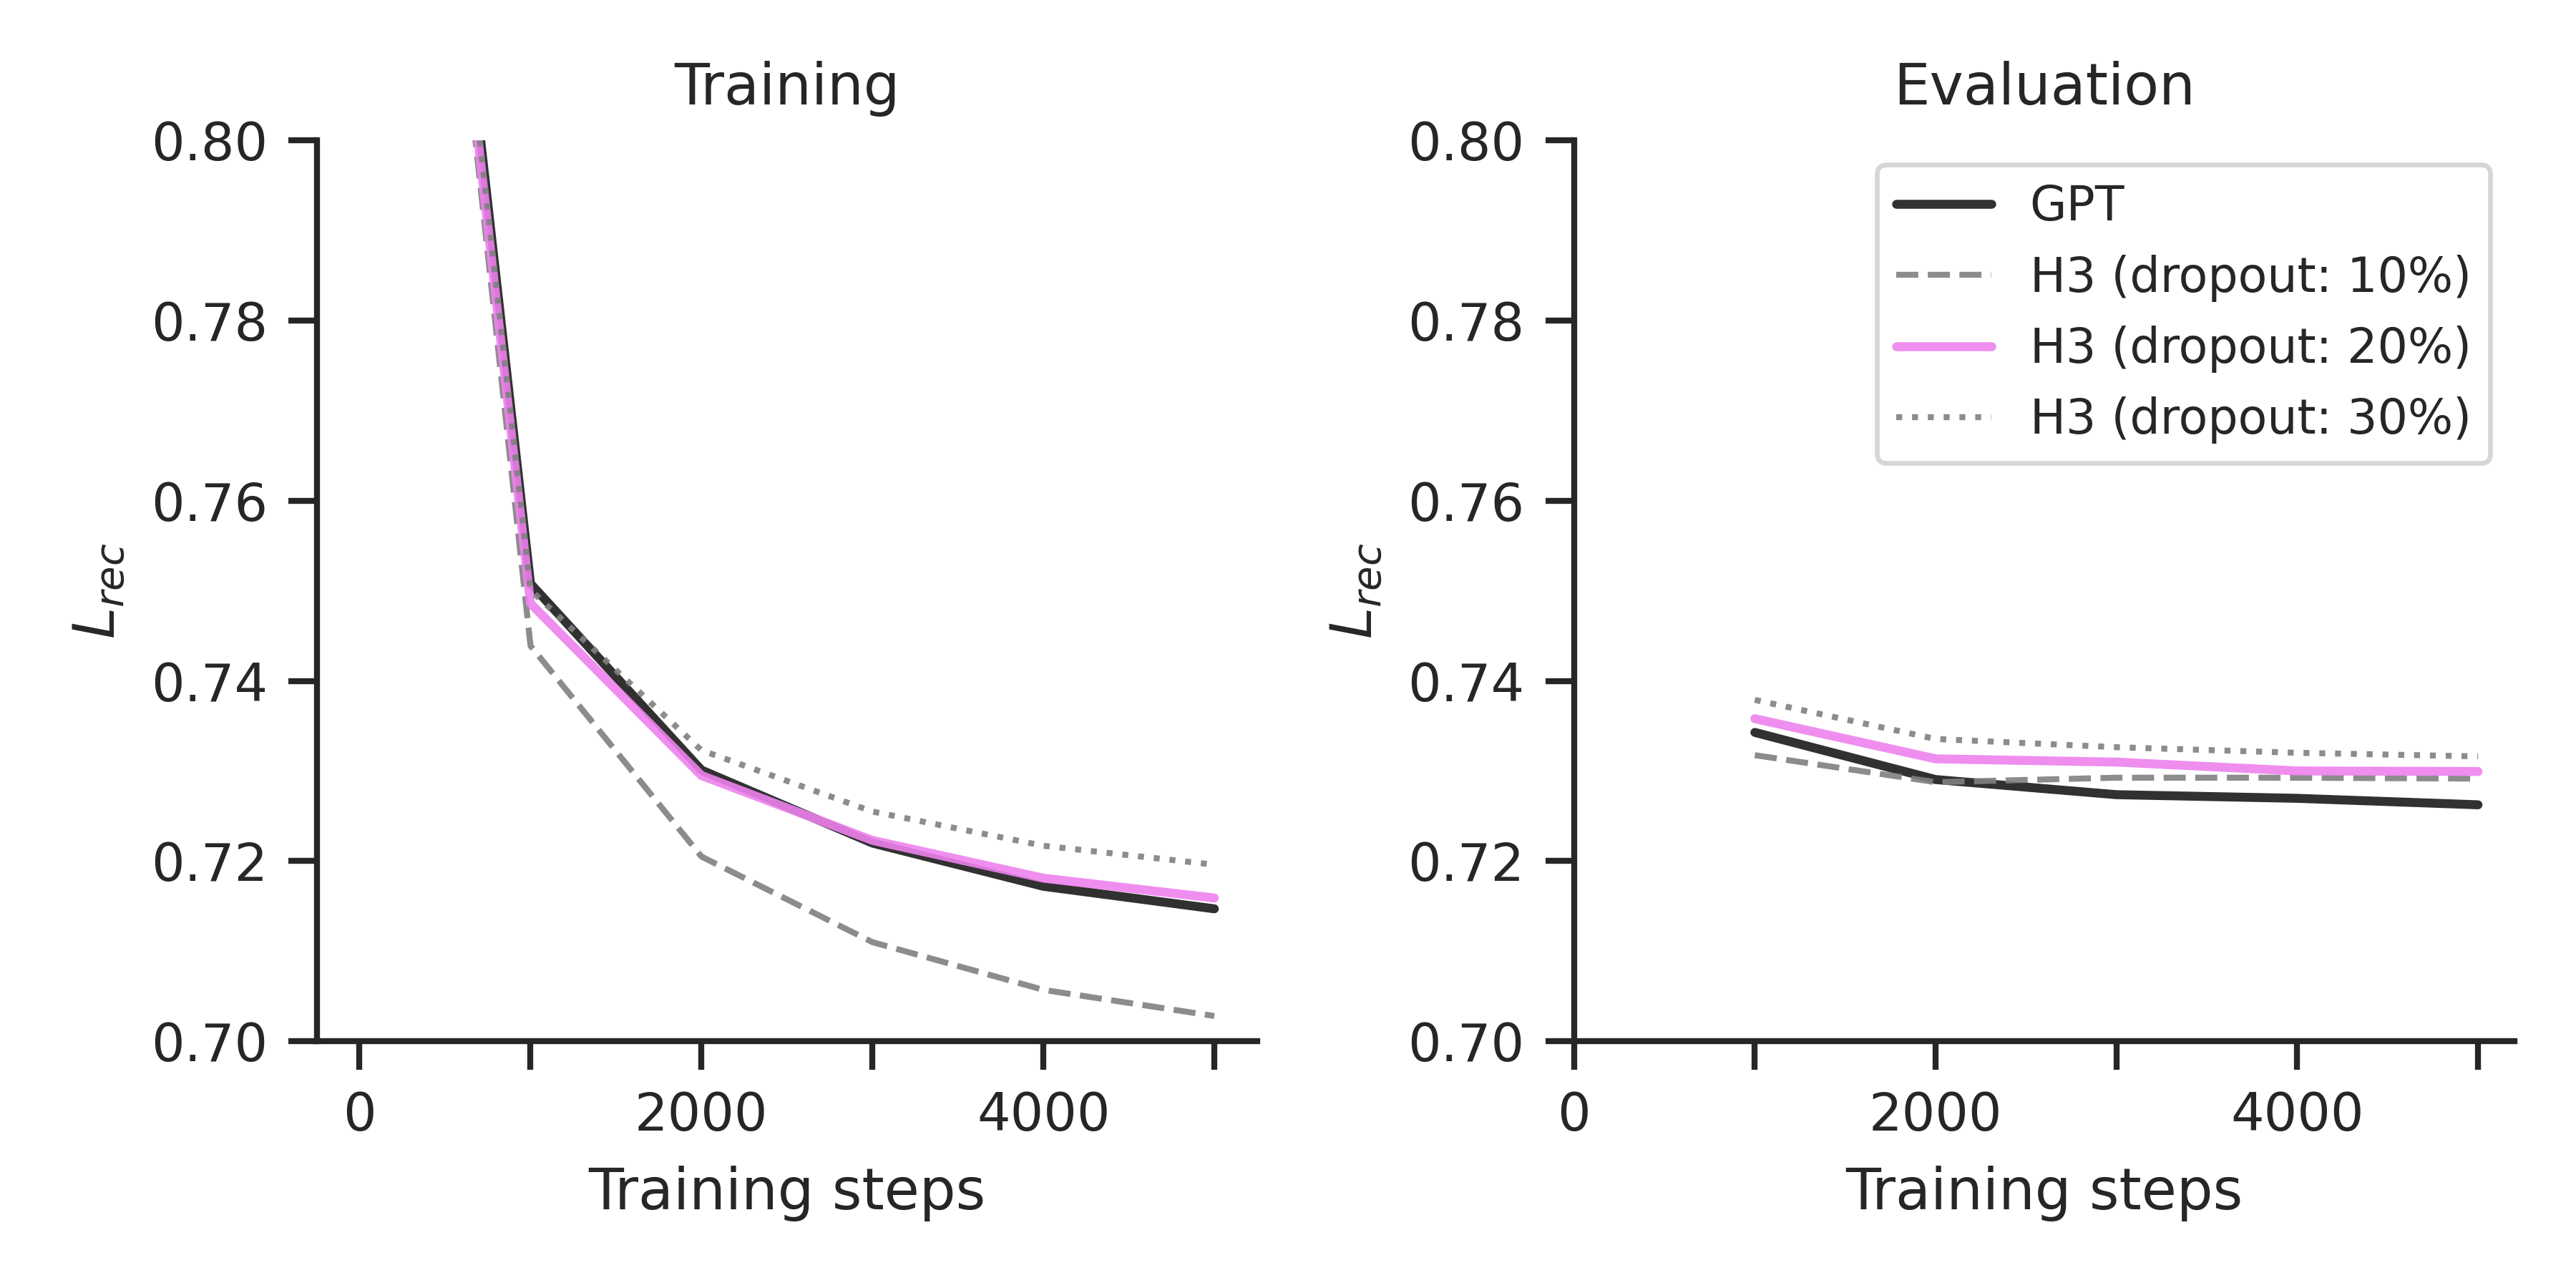
\includegraphics[width=0.65\textwidth]{figs/fmri_upstream-error.png}
    \caption{\label{fig:fmri-upstream} Upstream mean absolute error ($L_{rec}$) in training and evaluation datasets over the course of model training.}
\end{figure}

We find that the H3 variant trained with $0.2$ dropout performs on par with the GPT model, in terms of mean absolute error (Fig.\ \ref{fig:fmri-upstream}), and therefore continue all further analyses with this model variant. We also find that both models exhibit almost identify $L_{rec}$ error distributions throughout the brain, with relatively higher errors in the posterior parietal, occipital, and cingulate cortices as well parts of the limbic system (Fig.\ \ref{fig:fmri-upstream-brain}).

\begin{figure}[h]
    \centering
    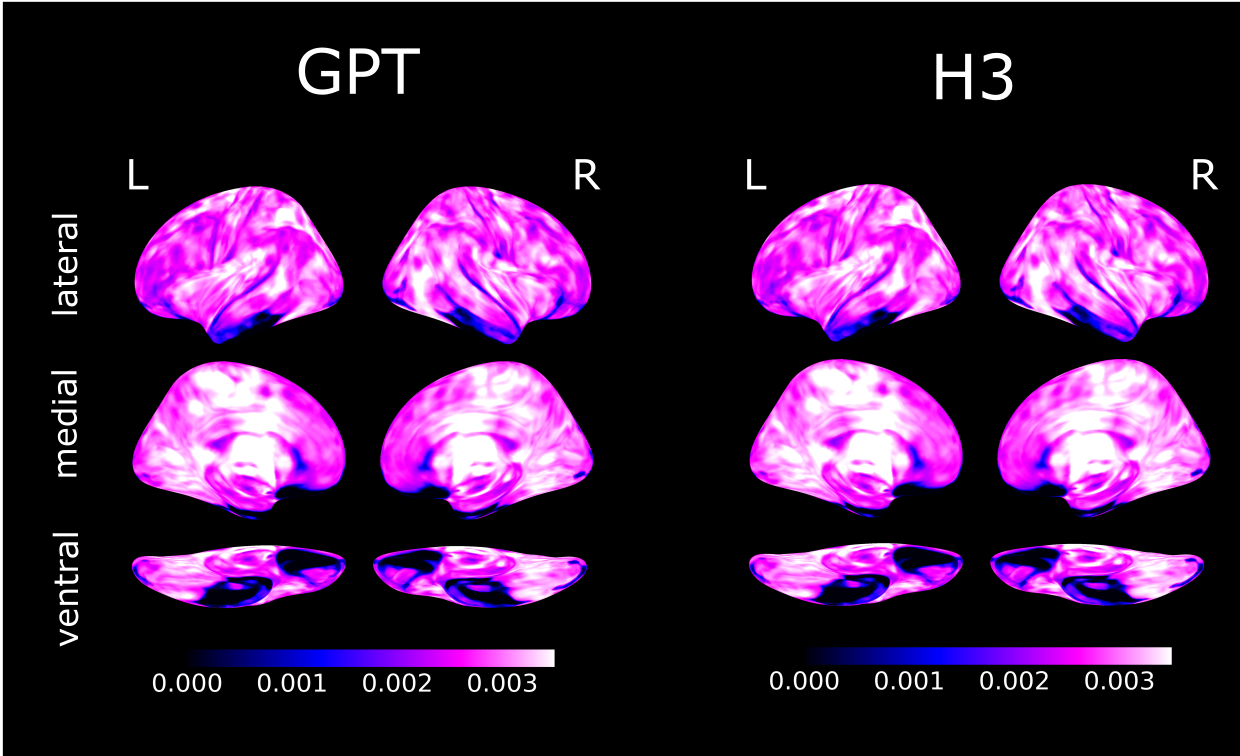
\includegraphics[width=0.5\textwidth]{figs/fmri_upstream-error-brain.png}
    \caption{\label{fig:fmri-upstream-brain} Mean absolute error ($L_{rec}$) of the final pre-trained models for each voxel of the brain projected onto the inflated cortical surface of the FsAverage template~\citep{fischl_2012_freesurfer}.}
\end{figure}

To adapt the pre-trained models to mental state decoding, we add a learnable classification embedding $E^{cls} \in \mathbb{R}^{n}$ to the end of input sequences $X$ and forward the model's prediction $f(E^{X})$ to a decoding head $p(\cdot)$, composed of a dense hidden layer with $e$ model units (one for each embedding dimension, with $tanh$ activation) as well as a $softmax$ output layer with one model unit $i$ for each considered mental state in the data. Accordingly, we adapt models by optimizing a standard cross entropy loss objective: $L_{cls} = - \sum_i y_i \log \ {p(f(E^X))_i}$, where $y_i$ indicates a binary variable that is $1$ if $i$ is the correct mental state and $0$ otherwise.

During downstream adaptation, we begin training with the respective pre-trained model parameters and then allow all parameters to change freely. Similar to~\citep{thomas_fmri_2022}, we randomly split each of the two downstream datasets into distinct training and test datasets, each comprising $40$ (HCP) or $10$ (MDTB) distinct individuals. We adapt models for $750$ steps at a mini-batch size of $256$ and a learning rate of $5e^{-5}$ (otherwise using the same learning parameters as for upstream training). Importantly, we repeat each downstream training run $20$ times using different random seeds, leading to different random splits of the data and variability in other non-deterministic training factors (such as random initialization and data shuffling).

As for the upstream data, the H3 and GPT-based models generally perform on par in their mental state decoding performances in the two left-out test datasets (Table \ref{table:fmri-downstream}).

\begin{table}[h]
    % \captionsetup{font=small}
    \small
    \centering
    %\vspace{-1em}
    \caption{\label{table:fmri-downstream} Downstream adaptation performance of models pre-trained on fMRI data, averaged over $20$ training runs with varying random seeds. F1-scores are macro-averaged.}
    %   \vspace{1em}
    {
        \begin{tabular}{@{}|c|c|cc|@{}}
        %   \specialrule{.15em}{.05em}{.05em}
        \hline
        Dataset & Model & Acc. ($\pm 95\% \text{CI}$) & F1 ($\pm 95\% \text{CI}$)\\ % & Training time \\
        %   \specialrule{.15em}{.05em}{.05em}
        \hline
        HCP & GPT & $88.44$ ($\pm 0.39$) & $87.24$ ($\pm 0.39$) \\
         & H3 & $88.75$ ($\pm 0.33$) & $87.16$ ($\pm 0.37$) \\ \hline
        MDTB & GPT & $89.47$ ($\pm 0.44$) & $88.74$ ($\pm 0.54$) \\
         & H3 & $88.25$ ($\pm 0.45$) & $85.76$ ($\pm 0.61$) \\ \hline
        \end{tabular}
    }
    %\vspace{-1em}
\end{table}

\end{document}
